% LaTeX source for textbook ``Think C++, a game perspective''
% Copyright (C) 2023  Lisa Patacchiola, Allen B. Downey


\DocumentMetadata{}
\documentclass{book}
\usepackage[pdftex,
            pdfauthor={Lisa Patacchiola and Allen B Downey},
            pdftitle={ThinkCPP, a game perspective},
            pdfsubject={Programming},
            pdfkeywords={c++, programming, games},
            pdfproducer={Latex with hyperref, or other system},
            pdfcreator={pdflatex, or other tool}]{hyperref}
\usepackage{makeidx}
\usepackage{url}
\usepackage{listings}
\usepackage{graphicx}
\graphicspath{ {./images/} }
\pssilent
%\usepackage[tagged, highstructure]{accessibility}
%\usepackage{tagpdf}
\usepackage{color}
\definecolor{dkgreen}{RGB}{46,133,64}
\definecolor{gray}{rgb}{0.5,0.5,0.5}
\definecolor{mauve}{rgb}{0.58,0,0.82}
\definecolor{lightblue}{rgb}{0.5, 0.6, 0.8}
\definecolor{mint}{RGB}{236, 253, 226}
\lstset{language=[ANSI]C++,
keywordstyle=\color{blue}\bfseries, % style for keywords
showstringspaces=false,
   commentstyle=\color{dkgreen},
   stringstyle=\color{mauve},
   basicstyle={\small\ttfamily},
   backgroundcolor=\color{mint}
}   
%\renewcommand\cftsecnumwidth{2em}

\title{Think C++, a game perspective}

\author{Lisa Patacchiola, Allen B. Downey (original author)}
\date{4/3/2023}

\sloppy
\setlength{\topmargin}{0.75in}
\setlength{\headsep}{0.5in}
\setlength{\oddsidemargin}{1.0in}
\setlength{\evensidemargin}{.95in}
\makeindex

\begin{document}

\title {Think C++, a game perspective}
\date {Version 2.0 alpha 0.8}
\maketitle

\vspace{2in}
\begin{center}
{\Large Think C++, a game perspective}

\vspace{0.25in}

Copyright (C) 2023 Lisa Patacchiola and Allen B. Downey
\end{center}
\vspace{0.25in}

Permission is granted to copy, distribute, transmit and adapt this
work under the Creative Commons Attribution-NonCommercial-ShareAlike 4.0
International License: \url{https://creativecommons.org/licenses/by-nc/4.0/}.

If you are interested in distributing a commercial version of this
work, please contact the author.

\bigskip
The \LaTeX\ source and code for this version of the book are available from

\bigskip
\url{https://github.com/lpatacch/thinkCPPGames}

\bigskip
The \LaTeX\ source and code for the original book is available from

\bigskip
\url{https://github.com/AllenDowney/ThinkCPP}



\frontmatter
% LaTeX source for textbook ``Think C++, a game perspective''
% Copyright (C) 2023  Lisa Patacchiola

\chapter{Preface}

\section{Notes from Lisa}
Hi! If you are reading this note, you are reading an alpha version of this book. That means that I have not completely converted the book over the the format I eventually want to have. Double check my github account that you have the most recent version.

If this is the most recent version, here is the information so far.

Chapter 1 and 2 has some work done. I have changed some of the examples to have more of a game flavor. I have moved Functions a bit further back in the book and have moved If statements up to Chapter 3. I have also brought switch statements up as well. Chapter 3 has been started, but has not been converted over yet. You will still find "FIXME"s in the chapter, and I have not switched the examples to something more game-like. I have put stubs for flowcharts and pseudo code, but I have not put anything in there yet. Other chapters have had small changes, mostly so the previous links are no longer broken.

I have added an appendix to talk about how to turn on warnings on Replit.


More notes:

I was previously using a different book for my classes. It did have lots of information, but it seemed like it had too much information. Students couldn't get through the reading because they found it too long and complex.

I started to use ThinkCPP, but I noticed that the book was using various coding practices that were no longer acceptable. (They were perfect when it was published, but C++ has changed a bit since then.) I first was only going to change a few examples, but after a few student questions, I decided to do a larger change to this book.


\section{Acknowledgments}

\section{Contributions}
The first edition was called "Think like a computer scientist" and was written by Allen B. Downey. 

Lisa Patacchiola wrote the new additions and created Replit projects for the examples. 



\tableofcontents

\mainmatter
% LaTeX source for textbook ``ThinkCPP , a game perspective''
% Copyright (C) 2023  Lisa Patacchiola and Allen B. Downey


\chapter{The way of the program}

The goal of this book is to teach you to think like a
computer scientist.  I like the way computer scientists think because
they combine some of the best features of Mathematics, Engineering,
and Natural Science.  Like mathematicians, computer scientists use formal
languages to denote ideas (specifically computations).  Like
engineers, they design things, assembling components into systems and
evaluating trade-offs among alternatives.  Like scientists,
they observe the behavior of complex systems, form hypotheses, and test
predictions.

The single most important skill for a computer scientist is {\bf
problem-solving}.  By that I mean the ability to formulate problems,
think creatively about solutions, and express a solution clearly and
accurately.  As it turns out, the process of learning to program is an
excellent opportunity to practice problem-solving skills.  That's why
this chapter is called ``The way of the program.''

\section{What is a programming language?}
\index{programming language}
\index{language!programming}

The programming language you will be learning is C++, because it is used 
in many video games and in the Unreal Engine. Both C++ and C\# are
 {\bf high-level languages}; other high-level languages you might have 
heard of are Java, C and Python.

As you might infer from the name ``high-level language,'' there are
also {\bf low-level languages}, sometimes referred to as machine
language or assembly language.  Loosely-speaking, computers can only
execute programs written in low-level languages.  Thus, programs
written in a high-level language have to be translated before they can
run.  This translation takes some time, which is a small disadvantage
of high-level languages.

\index{portability}
\index{high-level language}
\index{low-level language}
\index{language!high-level}
\index{language!low-level}

But the advantages are enormous.  First,
it is {\em much} easier to program in a high-level language;
by ``easier'' I mean that the program takes less time to write,
it's shorter and easier to read, and it's more likely to be
correct.  Secondly, high-level languages are {\bf portable},
meaning that they can run on different kinds of computers with
few or no modifications.  Low-level programs can only run
on one kind of computer, and have to be rewritten to run on
another.

Due to these advantages, almost all programs are written in
high-level languages.  Low-level languages are only used for
a few special applications.

\index{compile}
\index{interpret}

There are two ways to translate a program; {\bf interpreting} or {\bf
compiling}.  An interpreter is a program that reads a high-level
program and does what it says.  In effect, it translates the program
line-by-line, alternately reading lines and carrying out commands.

\vspace{0.1in}
\centerline{\epsfig{figure=interpret.eps}}
\vspace{0.1in}

A compiler is a program that reads a high-level program and
translates it all at once, before executing any of the commands.
Often you compile the program as a separate step, and then
execute the compiled code later.  In this case, the high-level
program is called the {\bf source code}, and the translated
program is called the {\bf object code} or the {\bf executable}.

As an example, suppose you write a program in C++.  You might
use a text editor to write the program (a text editor is
a simple word processor).  When the program is finished, you
might save it in a file named {\tt program.cpp}, where ``program''
is an arbitrary name you make up, and the suffix {\tt .cpp} is
a convention that indicates that the file contains C++ source
code.

Then, depending on what your programming environment is like,
you might leave the text editor and run the compiler.  The
compiler would read your source code, translate it, and create
a new file named {\tt program.o} or {\tt program.obj} to contain the object code,
and {\tt program.out} or {\tt program.exe} to contain the executable. 

\vspace{0.1in}
\centerline{\epsfig{figure=compile.eps}}
\vspace{0.1in}

The next step is to run the program, which requires some kind
of executor.  The role of the executor is to load the program
(copy it from disk into memory) and make the computer start
executing the program.

Although this process may seem complicated, the good news is that in
most programming environments (sometimes called integrated development
environments(IDE)), these steps are automated for you.  Usually you will
only have to write a program and type a single command to compile and
run it.  On the other hand, it is useful to know what the steps are
that are happening in the background so that if something goes wrong,
you can figure out what it is.

\index{replit}
The longer code examples in this book will use Replit.com, an online programming
platform/IDE, and community. Code listings include links to the “repl” that you can copy 
(“fork”) and experiment with.

\section{What is a program?}

A program is a sequence of instructions that specifies how to perform
a computation.  The computation might be something mathematical, like
solving a system of equations or finding the roots of a polynomial,
but it can also be a symbolic computation, like searching and
replacing text in a document or (strangely enough) compiling a
program. Or, it could be something fun, like a character trying to walk around and find a dragon. All of these things can be done with a program.

\index{statement}

The instructions (or commands, or statements) look different in
different programming languages, but there are a few basic functions
that appear in just about every language:

\begin{description}

\index{input}
\item[input:] Get data from the keyboard, or a file, or some
other device.

\index{output}
\item[output:] Display data on the screen or send data to a
file or other device.

\index{math}
\index{processing}
\item[math:] Perform basic mathematical operations like addition and
multiplication. (Sometimes called "Processing")

\index{testing}
\index{selection}
\item[testing:] Check for certain conditions and execute the
appropriate sequence of statements. (Sometimes called "Selection")

\index{iteration}
\index{repetition}
\index{loop}
\item[repetition:] Perform some action repeatedly, usually with
some variation. (Sometimes called "Iteration" or "looping")

\end{description}

Believe it or not, that's pretty much all there is to it.
Every program you've ever used, no matter how complicated, is
made up of functions that look more or less like these.  Thus,
one way to describe programming is the process of breaking a
large, complex task up into smaller and smaller subtasks
until eventually the subtasks are simple enough to be performed
with one of these simple functions.

\section{What is debugging?}
\index{debugging}
\index{bug}

Programming is a complex process, and since it is done by
human beings, it often leads to errors.  For whimsical reasons,
programming errors are called {\bf bugs} and the process
of tracking them down and correcting them is called
{\bf debugging}.

There are a few different kinds of errors that can occur
in a program, and it is useful to distinguish between them
in order to track them down more quickly.

\subsection{Compile-time errors}
\index{compile-time error}
\index{error!compile-time}
\index{error!syntax}
\index{syntax error}

The compiler can only translate a program if the program is
syntactically correct; otherwise, the compilation fails and
you will not be able to run your program.  {\bf Syntax}
refers to the structure of your program and the rules about
that structure. A mistake with the syntax is often called a {\bf syntax error}.

\index{syntax}

For example, in English, a sentence must begin with a capital
letter and end with a period.  this sentence contains a syntax
error.  So does this one

For most readers, a few syntax errors are not a significant
problem, which is why we can read the poetry of e e cummings
without spewing error messages.

Compilers are not so forgiving.  If there is a single syntax
error anywhere in your program, the compiler will print an
error message and quit, and you will not be able to run
your program.

To make matters worse, there are more syntax rules in C++
than there are in English, and the error messages you get from
the compiler are often not very helpful.  During the first
few weeks of your programming career, you will probably
spend a lot of time tracking down syntax errors.  As you
gain experience, though, you will make fewer errors and find
them faster.

When you get a syntax error, don't think that the compiler is yelling at you for getting something wrong. Think of it ask asking you for help. "Help" it is saying "I have no idea what this means, please help me". Honestly, I like syntax errors more than any of the other types of errors. Syntax errors are one of the few errors where the computer tells you it found a problem and suggests what it thinks is wrong. 
\subsection{Run-time errors}
\label{run-time}
\index{run-time error}
\index{error!run-time}
\index{safe language}
\index{language!safe}

The second type of error is a run-time error, so-called because
the error does not appear until you run the program.

For the simple sorts of programs we will be writing for the
next few weeks, run-time errors are rare, so it might be a little
while before you encounter one.


\subsection{Logic errors and semantics}
\index{semantics}
\index{logic error}
\index{error!logic}

The third type of error is the {\bf logical} or {\bf semantic}
error.  If there is a logical error in your program, it will
compile and run successfully, in the sense that the computer
will not generate any error messages, but it will not do the
right thing.  It will do something else.  Specifically, it will
do what you told it to do.

The problem is that the program you wrote is not the program
you wanted to write.  The meaning of the program (its semantics)
is wrong.  

Let's say you have a program that tells the computer to do the following steps:
\begin{enumerate}
    \item Get the pitcher of water
    \item Pour the water
    \item Get the glass
\end{enumerate}
A person would see that list and would assume you meant to get the glass first. The computer would do exactly as you asked and spill water on the table and then put a glass on top. There was an obvious logical error in your program, but it ran without a compile error. As far as the computer was concerned, it ran perfectly. But, you know that was not your original intent.

Identifying logical errors can be tricky, since
it requires you to work backwards by looking at the output
of the program and trying to figure out what it is doing.

\subsection{Experimental debugging}

One of the most important skills you should acquire from working with
this book is debugging.  Although it can be frustrating, debugging is
one of the most intellectually rich, challenging, and interesting
parts of programming.

In some ways debugging is like detective work.  You are
confronted with clues and you have to infer the processes
and events that lead to the results you see.

Debugging is also like an experimental science.  Once you have an idea
what is going wrong, you modify your program and try again.  If your
hypothesis was correct, then you can predict the result of the
modification, and you take a step closer to a working program.  If
your hypothesis was wrong, you have to come up with a new one.  As
Sherlock Holmes pointed out, ``When you have eliminated the
impossible, whatever remains, however improbable, must be the truth.''
(from A. Conan Doyle's {\em The Sign of Four}).

\index{Holmes, Sherlock}
\index{Doyle, Arthur Conan}

For some people, programming and debugging are the
same thing.  That is, programming is the process of gradually
debugging a program until it does what you want.  The idea
is that you should always start with a working program that
does {\em something}, and make small modifications, debugging
them as you go, so that you always have a working program.

For example, Linux is an operating system that contains thousands of
lines of code, but it started out as a simple program Linus Torvalds
used to explore the Intel 80386 chip.  According to Larry Greenfield,
``One of Linus's earlier projects was a program that would switch
between printing AAAA and BBBB.  This later evolved to Linux''
(from {\em The Linux Users' Guide} Beta Version 1).

\index{Linux}

In later chapters I will make more suggestions about debugging
and other programming practices.

\section{Formal and natural languages}
\label{formal}
\index{formal language}
\index{natural language}
\index{language!formal}
\index{language!natural}

{\bf Natural languages} are the languages that people speak,
like English, Spanish, and French.  They were not designed
by people (although people try to impose some order on them);
they evolved naturally.

{\bf Formal languages} are languages that are designed by people for
specific applications.  For example, the notation that mathematicians
use is a formal language that is particularly good at denoting
relationships among numbers and symbols.  Chemists use a formal
language to represent the chemical structure of molecules.  And
most importantly:

\begin{quote}
{\bf Programming languages are formal languages that have been
designed to express computations.}
\end{quote}

As I mentioned before, formal languages tend to have strict rules
about syntax.  For example, $3+3=6$ is a syntactically correct
mathematical statement, but $3=+6\$$ is not.  Also, $H_2O$ is a
syntactically correct chemical name, but $_2Zz$ is not.

Syntax rules come in two flavors, pertaining to tokens and structure.
Tokens are the basic elements of the language, like words and numbers
and chemical elements.  One of the problems with {\tt 3=+6\$} is that
{\tt \$} is not a legal token in mathematics (at least as far as I
know).  Similarly, $_2Zz$ is not legal because there is no element with
the abbreviation $Zz$.

The second type of syntax error pertains to the structure of a
statement; that is, the way the tokens are arranged.  The statement
{\tt 3=+6\$} is structurally illegal, because you can't have a plus
sign immediately after an equals sign.  Similarly, molecular formulas
have to have subscripts after the element name, not before.

When you read a sentence in English or a statement in a formal
language, you have to figure out what the structure of the sentence is
(although in a natural language you do this unconsciously).  This
process is called {\bf parsing}.

\index{parse}

For example, when you hear the sentence, ``The other shoe fell,'' you
understand that ``the other shoe'' is the subject and ``fell'' is the
verb.  Once you have parsed a sentence, you can figure out what it
means, that is, the semantics of the sentence.  Assuming that you know
what a shoe is, and what it means to fall, you will understand the
general implication of this sentence.

Although formal and natural languages have many features in
common---tokens, structure, syntax and semantics---there are many
differences.

\index{ambiguity}
\index{redundancy}
\index{literalness}

\begin{description}

\item[ambiguity:] Natural languages are full of ambiguity, which
people deal with by using contextual clues and other information.
Formal languages are designed to be nearly or completely unambiguous,
which means that any statement has exactly one meaning,
regardless of context.

\item[redundancy:] In order to make up for ambiguity and reduce
misunderstandings, natural languages employ lots of
redundancy.  As a result, they are often verbose.  Formal languages
are less redundant and more concise.

\item[literalness:] Natural languages are full of idiom and
metaphor.  If I say, ``The other shoe fell,'' there is probably
no shoe and nothing falling.  Formal languages mean
exactly what they say.

\end{description}

People who grow up speaking a natural language (everyone) often have a
hard time adjusting to formal languages.  In some ways the difference
between formal and natural language is like the difference between
poetry and prose, but more so:

\index{poetry}
\index{prose}

\begin{description}

\item[Poetry:] Words are used for their sounds as well as for
their meaning, and the whole poem together creates an effect or
emotional response.  Ambiguity is not only common but often
deliberate.

\item[Prose:] The literal meaning of words is more important
and the structure contributes more meaning.  Prose is more amenable to
analysis than poetry, but still often ambiguous.

\item[Programs:] The meaning of a computer program is unambiguous
and literal, and can be understood entirely by analysis of the
tokens and structure.

\end{description}

Here are some suggestions for reading programs (and other formal
languages).  First, remember that formal languages are much more dense
than natural languages, so it takes longer to read them.  Also, the
structure is very important, so it is usually not a good idea to read
from top to bottom, left to right.  Instead, learn to parse the
program in your head, identifying the tokens and interpreting the
structure.  Finally, remember that the details matter.  Little things
like spelling errors and bad punctuation, which you can get away
with in natural languages, can make a big difference in a formal
language.

\section{The first program}
\label{hello}
\index{hello world}

Traditionally the first program people write in a new language
is called ``Hello, World.'' because all it does is print the
words ``Hello, World.''  In C++, this program looks like this:


\begin{lstlisting}[frame=single]
#include <iostream>

// main: generate some simple output

int main ()
{
  std::cout << "Hello, world." << std::endl;
  return 0;
}
\end{lstlisting}
%

Some people judge the quality of a programming language by
the simplicity of the ``Hello, World.'' program.  By this
standard, C++ does reasonably well.  Even so, this simple
program contains several features that are hard to explain to
beginning programmers.  For now, we will ignore some of
them, like the first line.

\index{comment}
\index{statement!comment}

The third line begins with {\tt //}, which indicates
that it is a {\bf comment}.  A comment is a bit of
English text that you can put in the middle of a program,
usually to explain what the program does.  When the compiler
sees a {\tt //}, it ignores everything from there until the end
of the line.

In the fourth line, you can ignore the word {\tt int}
for now, but notice the word {\tt main}.  {\tt main} is a
special name that indicates the place in the program where execution
begins.  When the program runs, it starts by executing the first
statement in {\tt main} and it continues, in order, until it gets
to the last statement, and then it quits.

\index{output}
\index{statement!output}

There is no limit to the number of statements that can be in {\tt
main}, but the example contains only one.  It is a basic {\bf
output} statement, meaning that it outputs or displays a message on
the screen.  

{\tt std::cout} is a special object provided by the system to allow
you to send output to the screen.  The symbol {\tt <<} is an
{\bf operator} that you apply to {\tt std::cout} and a string, and that
causes the string to be displayed.

\index{operator}

{\tt std::endl} is a special symbol that represents the end of a
line.  When you send an {\tt std::endl} to {\tt std::cout}, it causes the
cursor to move to the next line of the display.
The next time you output something, the new text appears
on the next line. (Note: the word is endl ends with an L, not a 1.)

Like all statements, the output statement ends with a
semi-colon ({\tt ;}).

There are a few other things you should notice about the syntax of
this program.  First, C++ uses squiggly-braces (\{ and
\}) to group things together.  In this case, the output statement
is enclosed in squiggly-braces, indicating that it is {\em inside} the
definition of {\tt main}.  Also, notice that the statement is
indented, which helps to show visually which lines are inside the
definition.

At this point it would be a good idea to sit down in front of
a computer and compile and run this program.  

To try program out, go to:
\url{https://replit.com/@lpatacch/helloWorld#hello.cpp}

\index{replit}
When the project is loaded, you should see a button that looks like Figure \ref{fig:Run}.
\smallskip
\begin{figure}
    \centering
    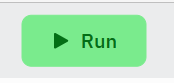
\includegraphics{Run}
    \caption{The Run button on Replit}
    \label{fig:Run}
\end{figure}

If you click that "Run" button, it will compile the code and run it. You should see the words "Hello World!" on the right side of the environment. Congratulations! You just created your first program!

As I mentioned, the C++ compiler is a real stickler for syntax.
If you make any errors when you type in the program, chances
are that it will not compile successfully.  For example, if
you misspell {\tt iostream}, you might get an error message like
the following:

\begin{verbatim}
hello.cpp:1: oistream.h: No such file or directory
\end{verbatim}
%
There is a lot of information on this line, but it is presented
in a dense format that is not easy to interpret.  A more friendly
compiler might say something like:

\begin{quote}
``On line 1 of the source code file named hello.cpp, you tried to
include a header file named oistream.h.  I didn't find anything
with that name, but I did find something named iostream.  Is
that what you meant, by any chance?''
\end{quote}

Unfortunately, few compilers are so accommodating.  The compiler
is not really very smart, and in most cases the error message
you get will be only a hint about what is wrong.  It will take
some time to gain facility at interpreting compiler messages.

Nevertheless, the compiler can be a useful tool for learning the
syntax rules of a language.  Starting with a working program
(like hello.cpp), modify it in various ways and see what happens.
If you get an error message, try to remember what the message says
and what caused it, so if you see it again in the future you
will know what it means.

\section{Exercises}
FIXME
Hello, I got this running (modified hello world)

\section{Glossary}

\begin{description}

\item[problem-solving:]  The process of formulating a problem, finding
a solution, and expressing the solution.

\item[high-level language:]  A programming language like C++ that
is designed to be easy for humans to read and write.

\item[low-level language:]  A programming language that is designed
to be easy for a computer to execute.  Also called ``machine
language'' or ``assembly language.''

\item[portability:]  A property of a program that can run on more
than one kind of computer.

\item[formal language:]  Any of the languages people have designed
for specific purposes, like representing mathematical ideas or
computer programs.  All programming languages are formal languages.

\item[natural language:]  Any of the languages people speak that
have evolved naturally.

\item[interpret:]  To execute a program in a high-level language
by translating it one line at a time.

\item[compile:]  To translate a program in a high-level language
into a low-level language, all at once, in preparation for later
execution.

\item[source code:]  A program in a high-level language, before
being compiled.

\item[object code:]  The output of the compiler, after translating
the program.

\item[executable:]  Another name for object code that is ready
to be executed.

\item[algorithm:]  A general process for solving a category of
problems. 

\item[bug:]  An error in a program.

\item[syntax:]  The structure of a program.

\item[semantics:]  The meaning of a program.

\item[parse:]  To examine a program and analyze the syntactic structure.

\item[syntax error:]  An error in a program that makes it impossible
to parse (and therefore impossible to compile).

\item[run-time error:]  An error in a program that makes it fail at
run-time.

\item[logical error:]  An error in a program that makes it do something
other than what the programmer intended.

\item[debugging:]  The process of finding and removing any of
the three kinds of errors.

\index{problem-solving}
\index{high-level language}
\index{low-level language}
\index{formal language}
\index{natural language}
\index{interpret}
\index{compile}
\index{syntax}
\index{semantics}
\index{parse}
\index{error}
\index{debugging}

\end{description}




% LaTeX source for textbook ``How to think like a computer scientist''
% Copyright (C) 2023  Lisa Patacchiola and Allen B Downey


\chapter{Variables and types}

\section{More output}
\index{output}
\index{statement!output}

As I mentioned in the last chapter, you can put as many statements as
you want in {\tt main}.  For example, to output more than one line:

\begin{mdframed}
\begin{verbatim}
#include <iostream>

// main: generate some simple output

int main ()
{
  std::cout << "Hello, world." << std::endl; // output 1 line
  std::cout << "How are you?" << std::endl;  // output 1 more
  return 0;
}
\end{verbatim}
%
\end{mdframed}

As you can see, it is legal to put comments at the
end of a line, as well as on a line by themselves.

If you want to try that with the replit code, go back to the link from the last chapter 
\url{https://replit.com/@lpatacch/helloWorld#hello.cpp}. Then, look for a button on the right hand of the screen with the words "Fork Repl". It should look like Figure \ref{fig:fork}
\begin{figure}
    \centering
    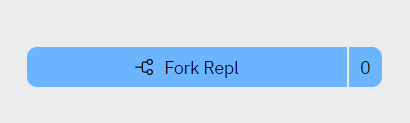
\includegraphics{fork}
    \caption{The Fork button on Replit}
    \label{fig:fork}
\end{figure}
You now should have a copy of the code that you can change any way you want.

\index{string}
\index{type!string}

In the program. the phrases that appear in quotation marks are called {\bf strings},
because they are made up of a sequence (string) of letters.  Actually,
strings can contain any combination of letters, numbers, punctuation
marks, and other special characters.

\index{newline}

Often it is useful to display the output from multiple output
statements all on one line.  You can do this by leaving out
the first {\tt endl}:

\begin{mdframed}

\begin{verbatim}
int main ()
{
  std::cout << "Goodbye, ";
  std::cout << "cruel world!" << std::endl;
  return 0
}
\end{verbatim}
%
\end{mdframed}
In this case the output appears on a single line as
{\tt Goodbye, cruel world!}.  Notice that there is a space
between the word ``Goodbye,'' and the second quotation mark.
This space appears in the output, so it affects the behavior
of the program.

Spaces that appear outside of quotation marks generally do
not affect the behavior of the program.  For example, I
could have written:

\begin{mdframed}

\begin{verbatim}
int main ()
{
  std::cout<<"Goodbye, ";
  std::cout<<"cruel world!"<<std::endl;
  return 0;
}
\end{verbatim}
%
\end{mdframed}
This program would compile and run just as well as the original.
The breaks at the ends of lines (newlines) do not affect
the program's behavior either, so I could have written:

\begin{mdframed}

\begin{verbatim}
int main(){std::cout<<"Goodbye, ";std::cout<<"cruel world!"
    <<std::endl;return 0;}
\end{verbatim}
%
\end{mdframed}
That would work, too, although you have probably noticed that
the program is getting harder and harder to read.  Newlines and
spaces are useful for organizing your program visually, making
it easier to read the program and locate syntax errors.

\section{Values}
\index{value}
\index{type}

A value is one of the fundamental things---like a letter or
a number---that a program manipulates.  The only values we have
manipulated so far are the string values we have been outputting, like
{\tt "Hello, world."}.  You (and the compiler) can identify
string values because they are enclosed in quotation marks.

There are other kinds of values, including integers and characters.
An integer is a whole number like 1 or 17.  You can output
integer values the same way you output strings:

\begin{mdframed}

\begin{verbatim}
  std::cout << 17 << std::endl;
\end{verbatim}
%

\end{mdframed}
A character value is a letter or digit or punctuation mark
enclosed in single quotes, like {\tt 'a'} or {\tt '5'}.
You can output character values the same way:


\begin{mdframed}

\begin{verbatim}
  std::cout << '}' << std::endl;
\end{verbatim}
%

\end{mdframed}
This example outputs a single close squiggly-brace on a line
by itself.

It is easy to confuse different types of values, like {\tt "5"}, {\tt
'5'} and {\tt 5}, but if you pay attention to the punctuation, it
should be clear that the first is a string, the second is a character
and the third is an integer.  The reason this distinction is important
should become clear soon.

\section {Variables}
\index{variable}
\index{value}

One of the most powerful features of a programming language is the
ability to manipulate {\bf variables}.  A variable is a named location
that stores a value.  

Just as there are different types of values (integer, character,
etc.), there are different types of variables.  When you create a new
variable, you have to declare what type it is.  For example, the
character type in C++ is called {\tt char}.  The following statement
creates a new variable named {\tt fred} that has type {\tt char}.

\begin{mdframed}

\begin{verbatim}
    char fred;
\end{verbatim}
%

\end{mdframed}
This kind of statement is called a {\bf declaration}.

The type of a variable determines what kind of values it can
store.  A {\tt char} variable can contain characters, and it should
come as no surprise that {\tt int} variables can store integers.

There are several types in C++ that can store string values, but we
are going to skip that for now (see Chapter~\ref{strings}).

\index{declaration}
\index{statement!declaration}

To create an integer variable, the syntax is 

\begin{mdframed}

\begin{verbatim}
  int bob;
\end{verbatim}
%

\end{mdframed}
where {\tt bob} is the arbitrary name you made up for the
variable.  In general, you will want to make up variable names
that indicate what you plan to do with the variable.  For
example, if you saw these variable declarations:

\begin{mdframed}

\begin{verbatim}
    char firstLetter;
    char lastLetter;
    int hour, minute;
\end{verbatim}
\end{mdframed}
%

you could probably make a good guess at what values
would be stored in them.  This example
also demonstrates the syntax for declaring multiple variables
with the same type: {\tt hour} and {\tt minute}
are both integers ({\tt int} type).

\section{Assignment}
\index{assignment}
\index{statement!assignment}

Now that we have created some variables, we would like to
store values in them.  We do that with an {\bf assignment
statement}.

\begin{mdframed}

\begin{verbatim}
    firstLetter = 'a';   // give firstLetter the value 'a'
    hour = 11;           // assign the value 11 to hour
    minute = 59;         // set minute to 59
\end{verbatim}
\end{mdframed}
%
This example shows three assignments, and the comments show
three different ways people sometimes talk about assignment
statements.  The vocabulary can be confusing here, but the
idea is straightforward:

\begin{itemize}

\item When you declare a variable, you create a named storage location.

\item When you make an assignment to a variable, you give it a value.

\end{itemize}

A common way to represent variables on paper is to draw a box
with the name of the variable on the outside and the value
of the variable on the inside.  This kind of figure is called
a {\bf state diagram} because is shows what state each of the
variables is in (you can think of it as the variable's ``state of
mind'').
This diagram shows
the effect of the three assignment statements:

\vspace{0.1in}
\centerline{\epsfig{figure=assign.eps}}
\vspace{0.1in}

\index{rules!variable value}
I sometimes use different shapes to indicate different
variable types.  These shapes should help remind you that one of the
rules in C++ is that a variable has to have the same type as the
value you assign it.  For example, you cannot store a string in
an {\tt int} variable.  The following statement generates a compiler
error.

\begin{mdframed}

\begin{verbatim}
  int hour;
  hour = "Hello.";       // WRONG !!
\end{verbatim}

\end{mdframed}
%
This rule is sometimes a source of confusion, because there are many
ways that you can convert values from one type to another, and C++
sometimes converts things automatically.  But for now you should
remember that as a general rule variables and values have the same
type, and we'll talk about special cases later.

Another source of confusion is that some strings {\em look}
like integers, but they are not.  For example,
the string {\tt "123"}, which is made up of the
characters {\tt 1}, {\tt 2} and {\tt 3}, is not
the same thing as the {\em number} {\tt 123}.
This assignment is illegal:

\begin{verbatim}
  minute = "59";         // WRONG!
\end{verbatim}
%
\section{Outputting variables}
\label{output}

You can output the value of a variable using the same commands
we used to output simple values.
\begin{mdframed}
\begin{verbatim}
  int hour, minute;
  char colon;

  hour = 11;
  minute = 59;
  colon = ':';

  std::cout << "The current time is ";
  std::cout << hour;
  std::cout << colon;
  std::cout << minute;
  std::cout << sts::endl;
\end{verbatim}
\end{mdframed}
%
Try this project here: \url{https://replit.com/@lpatacch/OutputVariables#main.cpp}.
This program creates two integer variables named {\tt hour} and {\tt
minute}, and a character variable named {\tt colon}.  It assigns
appropriate values to each of the variables and then uses a series
of output statements to generate the following:

\begin{verbatim}
The current time is 11:59
\end{verbatim}

When we talk about ``outputting a variable,'' we mean outputting the
{\em value} of the variable.  To output the {\em name} of a variable,
you have to put it in quotes.  For example: {\tt std::cout << "hour";}

As we have seen before, you can include more than one value in
a single output statement, which can make the previous program more
concise:

\begin{mdframed}

\begin{verbatim}
  int hour, minute;
  char colon;

  hour = 11;
  minute = 59;
  colon = ':';

  std::cout << "The current time is " << hour << colon 
                << minute << std::endl;
\end{verbatim}
\end{mdframed}
%
On one line, this program outputs a string, two integers, a character,
and the special value {\tt endl}.  Very impressive!


\section{Variable Naming Rules}
\index{variable naming rules}
\index{variable!naming rules}
\index{rules!variable naming}
A few sections ago, I said that you can make up any name you
want for your variables, but that's not quite true. There are certain rules that you need to follow.
\begin{enumerate}
    \item The name can not start with a number. (It is ok for a number to be in the name, it just can't be the first letter.)
    \item No spaces in the name
    \item Capitalization matters (num is different than NUM) 
    \item No special characters can be in the name other than underscore.
\end{enumerate}

Here are some examples of variables that do not follow the naming rules, and what you can use instead
\begin{mdframed}
\begin{verbatim}
    int 3player;    \\ WRONG, can not start with a number
    int player3;    \\ This would work
    int my3player   \\ This will also work
    
    int hit points; \\ WRONG, spaces not allowed in the name
    int hitPoints;  \\ This would work
    int hit_points; \\ This also would work
    
    int cash$;      \\ This would not work because of $sign
    int cashMoney;  \\ changed to use words instead
\end{verbatim}
\end{mdframed}
\subsection{Keywords}
\index{keyword}
In addition, there
are certain words that are reserved in C++ because they are
used by the compiler to parse the structure of your program,
and if you use them as variable names, it will get confused.
These words, called {\bf keywords}, include {\tt int},
{\tt char}, {\tt void}, {\tt endl} and many more.

The complete list of keywords is included in the C++ Standard, which
is the official language definition adopted by the the International
Organization for Standardization (ISO) on September 1, 1998.  You
can download a copy electronically from

    \url{http://www.ansi.org/}

%
Rather than memorize the list, I would suggest that you
take advantage of a feature provided in many development
environments: code highlighting.  As you type, different
parts of your program should appear in different colors.  For
example, keywords might be blue, strings red, and other code
black.  If you type a variable name and it turns blue, watch
out!  You might get some strange behavior from the compiler.

\section{Operators}
\index{operator}

{\bf Operators} are special symbols that are used to represent
simple computations like addition and multiplication.  Most
of the operators in C++ do exactly what you would expect them
to do, because they are common mathematical symbols.  For
example, the operator for adding two integers is {\tt +}.

The following are all legal C++ expressions whose meaning is
more or less obvious:

\begin{verbatim}
1+1        hour-1       hour*60 + minute     minute/60
\end{verbatim}
%
Expressions can contain both variables
names and integer values.  In each case the name of the variable is
replaced with its value before the computation is performed.

\index{expression}

\subsection{Not all the math operators}
Although some of the arithmetic operators that you would expect are there, there are some that do not work in C++. Here are a few examples of what does not work, and how to write it in a different way.

\begin{mdframed}
\begin{verbatim}
    int powerUpLevel = 2;
    int damageLevel = 3;
    
    int damageGiven = powerUpLeveldamageLevel;     // WRONG 
        // You can't just put variables next to each other
        // to have them multiply
        
    int damageGiven = powerUpLevel x damageLevel;  // WRONG 
        // You can't use x as a multiplication sign. It is
        // often used as a variable
        
    int damageGiven = powerUpLevel * damageLevel; // Correct!
        // When you multiply, you should use the * symbol
    
    int valToPower = powerUpLevel^2;              // WRONG
        // Although you can use the ^ symbol for a 
        // particular math operation, it is not to 
        // calculate the square (or any other power)
        // We will see this later in the book
        
    int valToPower = powerUpLevel * powerUpLevel; // Correct! 
        // To square a number, you can multiply it with
        // itself
        // There is also another way to do this which we
        // will see later
        
    int percentHurt = damageGiven ÷ 100;         // WRONG
        // C++ does not use this division sign
    
    int percentHurt = damageGiven/100;           // Correct
        // To divide, we should use the / symbol
        // There is something about this that is an issue,
        // that we will talk about right now.
\end{verbatim}
\end{mdframed}
%

\subsection{Integer Division}
Addition, subtraction and multiplication all do what you
expect, but you might be surprised by division.  For example,
the following program:

\begin{mdframed}

\begin{verbatim}
  int hour, minute;
  hour = 11;
  minute = 59;
  std::cout << "Number of minutes since midnight: ";
  std::cout << hour*60 + minute << std::endl;
  std::cout << "Fraction of the hour that has passed: ";
  std::cout << minute/60 << std::endl;
\end{verbatim}
\end{mdframed}
%

would generate the following output:

\begin{verbatim}
  Number of minutes since midnight: 719
  Fraction of the hour that has passed: 0
\end{verbatim}
%
Try it yourself here: \url{https://replit.com/@lpatacch/IntegerDivision#main.cpp}.
The first line is what we expected, but the second line is
odd.  The value of the variable {\tt minute} is 59, and
59 divided by 60 is 0.98333, not 0.  The reason for the
discrepancy is that C++ is performing {\bf integer division}.

\index{type!int}
\index{integer division}
\index{arithmetic!integer}
\index{division!integer}
\index{operand}

When both of the {\bf operands} are integers (operands are the things
operators operate on), the result must also be an integer,
and by definition integer division always rounds {\em down},
even in cases like this where the next integer is so close.

A possible alternative in this case is to calculate a percentage
rather than a fraction:

\begin{mdframed}
\begin{verbatim} 
  std::cout << "Percentage of the hour that has passed: ";
  std::cout << minute*100/60 << std::endl;
\end{verbatim}
\end{mdframed}

%
The result is:

\begin{verbatim}
    Percentage of the hour that has passed: 98
\end{verbatim}
%
Again the result is rounded down, but at least now the answer
is approximately correct.  In order to get an even more accurate
answer, we could use a different type of variable, called
floating-point, that is capable of storing fractional values.
We'll get to that in the next chapter.

\subsection{Modulus operator}
\label{modulus}
\index{modulus}
\index{remainder}
\index{operator!modulus}
\index{operator!remainder}
There is another way to get the information that the integer division is not using. That is a new operator called the {\bf modulus}, or {\bf remainder} operator.

The modulus operator works on integers (and integer expressions)
and yields the {\em remainder} when the first operand is divided
by the second.  In C++, the modulus operator is a percent sign,
{\tt \%}.  The syntax is exactly the same as for other operators:

\begin{verbatim}
  int quotient = 7 / 3;
  int remainder = 7 % 3;
\end{verbatim}
%
The first operator, integer division, yields 2.  The second
operator yields 1.  Thus, 7 divided by 3 is 2 with 1 left over.

The modulus operator turns out to be surprisingly useful.  For
example, you can check whether one number is divisible by
another: if {\tt x \% y} is zero, then {\tt x} is divisible
by {\tt y}.

Also, you can use the modulus operator to extract the rightmost
digit or digits from a number.  For example, {\tt x \% 10} yields
the rightmost digit of {\tt x} (in base 10).  Similarly
{\tt x \% 100} yields the last two digits.

\section{Order of operations}
\index{precedence}
\index{rules!precedence}
\index{order of operations}

When more than one operator appears in an expression the order
of evaluation depends on the rules of {\bf precedence}.  A
complete explanation of precedence can get complicated, but
just to get you started:

\begin{itemize}

\item Multiplication and division (and modulus) happen before
addition and subtraction.  So {\tt 2*3-1} yields 5, not 4, and {\tt
2/3-1} yields -1, not 1 (remember that in integer division {\tt 2/3}
is 0).

\item If the operators have the same precedence they are evaluated
from left to right.  So in the expression {\tt minute*100/60},
the multiplication happens first, yielding {\tt 5900/60}, which
in turn yields {\tt 98}.  If the operations had gone from right
to left, the result would be {\tt 59*1} which is {\tt 59}, which
is wrong.

\item Any time you want to override the rules of precedence (or
you are not sure what they are) you can use parentheses.  Expressions
in parentheses are evaluated first, so {\tt 2 * (3-1)} is 4.
You can also use parentheses to make an expression easier to
read, as in {\tt (minute * 100) / 60}, even though it doesn't
change the result.

\end{itemize}

\section{Operators for characters}
\index{character operator}
\index{operator!character}

Interestingly, the same mathematical operations that work on
integers also work on characters.  For example,

\begin{verbatim}
  char letter;
  letter = 'a' + 1;
  std::cout << letter << std::endl;
\end{verbatim}
%
outputs the letter {\tt b}.  Although it is syntactically legal
to multiply characters, it is almost never useful to do it.

Earlier I said that you can only assign integer values to
integer variables and character values to character variables,
but that is not completely true.  In some cases, C++ converts
automatically between types.  For example, the following is
legal.

\begin{verbatim}
  int number;
  number = 'a';
  std::cout << number << std::endl;
\end{verbatim}
%
The result is 97, which is the number that is used internally
by C++ to represent the letter {\tt 'a'}.  However, it is
generally a good idea to treat characters as characters, and
integers as integers, and only convert from one to the other
if there is a good reason.

Automatic type conversion is an example of a common problem in designing a
programming language, which is that there is a conflict between {\bf
formalism}, which is the requirement that formal languages should have
simple rules with few exceptions, and {\bf convenience}, which is the
requirement that programming languages be easy to use in practice.

More often than not, convenience wins, which is usually good for
expert programmers, who are spared from rigorous but unwieldy
formalism, but bad for beginning programmers, who are often baffled
by the complexity of the rules and the number of exceptions.  In this
book I have tried to simplify things by emphasizing the rules and
omitting many of the exceptions.


\section{Composition}
\index{composition}
\index{expression}

So far we have looked at the elements of a programming
language---variables, expressions, and statements---in
isolation, without talking about how to combine them.

One of the most useful features of programming languages
is their ability to take small building blocks and
{\bf compose} them.  For example, we know how to multiply
integers and we know how to output values; it turns out we can
do both at the same time:

\begin{verbatim}
    std::cout << 17 * 3;
\end{verbatim}
%
Actually, I shouldn't say ``at the same time,'' since in reality
the multiplication has to happen before the output, but
the point is that any expression, involving numbers, characters,
and variables, can be used inside an output statement.  We've
already seen one example:

\begin{verbatim}
  std::cout << hour*60 + minute << std::endl;
\end{verbatim}
%
You can also put arbitrary expressions on the right-hand
side of an assignment statement:

\begin{verbatim}
  int percentage;
  percentage = (minute * 100) / 60;
\end{verbatim}
%
This ability may not seem so impressive now, but we will see
other examples where composition makes it possible
to express complex computations neatly and concisely.

WARNING: There are limits on where you can use certain
expressions; most notably, the left-hand side of an assignment
statement has to be a {\em variable} name, not an expression.
That's because the left side indicates the storage location
where the result will go.  Expressions
do not represent storage locations, only values.  So the
following is illegal:  {\tt minute+1 = hour;}.

\section{Glossary}

\begin{description}

\item[variable:] A named storage location for values.  All
variables have a type, which determines which values it can
store.

\item[value:] A letter, or number, or other thing that can be
stored in a variable.  

\item[type:] A set of values.  The types
we have seen are integers ({\tt int} in C++) and characters ({\tt
char} in C++).

\item[keyword:]  A reserved word that is used by the compiler
to parse programs.  Examples we have seen include {\tt int},
{\tt void} and {\tt endl}.

\item[statement:] A line of code that represents a command or
action.  So far, the statements we have seen are declarations,
assignments, and output statements.

\item[declaration:] A statement that creates a new variable and
determines its type.

\item[assignment:] A statement that assigns a value to a variable.

\item[expression:] A combination of variables, operators and
values that represents a single result value.  Expressions also
have types, as determined by their operators and operands.

\item[operator:] A special symbol that represents a simple
computation like addition or multiplication.

\item[modulus:]  An operator that works on integers and yields
the remainder when one number is divided by another.  In C++
it is denoted with a percent sign ({\tt \%}).

\item[operand:] One of the values on which an operator operates. 

\item[precedence:] The order in which operations are evaluated.

\item[composition:] The ability to combine simple
expressions and statements into compound statements and expressions
in order to represent complex computations concisely.

\index{variable}
\index{value}
\index{type}
\index{keyword}
\index{statement}
\index{assignment}
\index{expression}
\index{operator}
\index{modulus}
\index{operand}
\index{composition}

\end{description}



% LaTeX source for textbook ``ThinkCPP , a game perspective''
% Copyright (C) 2023  Lisa Patacchiola, Allen B. Downey


\chapter{Conditionals}
\label{conditional}

\section{Floating-point}
\index{floating-point number}
\index{type!double}
\index{double (floating-point)}
\label{floating-point}

In the last chapter we had some problems dealing with numbers
that were not integers.  We worked around the problem by measuring
percentages instead of fractions, but a more general solution is
to use floating-point numbers, which can represent fractions
as well as integers.  In C++, there are two floating-point types,
called {\tt float} and {\tt double}.  In this book we will use
{\tt double}s exclusively.

You can create floating-point variables and assign values to them
using the same syntax we used for the other types.  For example:

\begin{lstlisting}
  double pi;
  pi = 3.14159;
\end{lstlisting}
%
It is also legal to declare a variable and assign a value to it at the
same time:

\begin{lstlisting}
  int x = 1;
  string empty = "";
  double pi = 3.14159;
\end{lstlisting}
%
In fact, this syntax is quite common.  A combined declaration
and assignment is sometimes called an {\bf initialization}.

\index{initialization}

Although floating-point numbers are useful, they are
often a source of confusion because there seems to be an
overlap between integers and floating-point numbers.  For
example, if you have the value {\tt 1}, is that an integer,
a floating-point number, or both?

Strictly speaking, C++ distinguishes the integer value {\tt 1}
from the floating-point value {\tt 1.0}, even though they
seem to be the same number.  They belong to
different types, and strictly speaking, you are not allowed
to make assignments between types.  For example, the following
is illegal

\begin{lstlisting}
    int x = 1.1;
\end{lstlisting}
%
because the variable on the left is an {\tt int}
and the value on the right is a {\tt double}.  But it is easy
to forget this rule, especially because there are places where C++
automatically converts from one type to another.
For example,

\begin{lstlisting}
    double y = 1;
\end{lstlisting}
%
should technically not be legal, but C++ allows it by converting the
{\tt int} to a {\tt double} automatically.  This leniency is
convenient, but it can cause problems; for example:

\begin{lstlisting}
    double y = 1 / 3;
\end{lstlisting}
%
You might expect the variable {\tt y} to be given the value
{\tt 0.333333}, which is a legal floating-point value, but in
fact it will get the value {\tt 0.0}.  The reason is that the
expression on the right appears to be the ratio of two integers,
so C++ does {\em integer} division, which yields the integer
value {\tt 0}.  Converted to floating-point, the result is
{\tt 0.0}.

One way to solve this problem (once you figure out what
it is) is to make the right-hand side a floating-point
expression:

\begin{lstlisting}
    double y = 1.0 / 3.0;
\end{lstlisting}
%
This sets {\tt y} to {\tt 0.333333}, as expected.

\index{arithmetic!floating-point}

All the operations we have seen---addition, subtraction,
multiplication, and division---work on floating-point values,
although you might be interested to know that the underlying mechanism
is completely different.  In fact, most processors have special
hardware just for performing floating-point operations.

\subsection{Converting from {\tt double} to {\tt int}}
\label{rounding}
\index{rounding}
\index{typecasting}
\index{static cast}
\index{cast!static}

As I mentioned, C++ converts {\tt int}s
to {\tt double}s automatically if necessary, because no
information is lost in the translation.  On the other hand,
going from a {\tt double} to an {\tt int} requires rounding
off.  C++ doesn't perform this operation automatically, in
order to make sure that you, as the programmer, are aware
of the loss of the fractional part of the number.

The simplest way to convert a floating-point value to an integer is to
use a {\bf typecast}.  Typecasting is so called because it allows you
to take a value that belongs to one type and ``cast'' it into another
type (in the sense of molding or reforming, not throwing).

The syntax for typecasting is different than code we have seen so far.  For example:

FIXME ADD more about STATIC CAST HERE
\begin{lstlisting}
  double pi = 3.14159;
  int x = static_cast<int>(pi);
\end{lstlisting}
%
The {\tt static\_cast<int>} function returns an integer, so {\tt x} gets the value
3.  Converting to an integer always rounds down, even if the fraction
part is 0.99999999.

For every type in C++, there is a corresponding function that
typecasts its argument to the appropriate type.

\section{Conditional execution}
\index{conditional}
\index{statement!conditional}

In order to write useful programs, we almost always need the ability
to check certain conditions and change the behavior of the program
accordingly.  {\bf Conditional statements} give us this ability.  The
simplest form is the {\tt if} statement:

\begin{lstlisting}
  if (x > 0) {
    std::cout << "x is positive" << std::endl;
  }
\end{lstlisting}
%
The expression in parentheses is called the condition.
If it is true, then the statements in brackets get executed.
If the condition is not true, nothing happens.

\index{operator!comparison}
\index{comparison!operator}

The condition can contain any of the {\tt comparison operators}:

\begin{lstlisting}
    x == y           // x equals y
    x != y           // x is not equal to y
    x > y            // x is greater than y
    x < y            // x is less than y
    x >= y           // x is greater than or equal to y
    x <= y           // x is less than or equal to y
\end{lstlisting}
%
Although these operations are probably familiar to you, the
syntax C++ uses is a little different from mathematical
symbols like $=$, $\neq$ and $\le$.  A common error is
to use a single {\tt =} instead of a double {\tt ==}.  Remember
that {\tt =} is the assignment operator, and {\tt ==} is
a comparison operator.  Also, there is no such thing as
{\tt =<} or {\tt =>}.

Unfortunately, the default behavior in many compilers is to not display warnings when you use one equal instead of two in an if statements. (Check out Chapter \ref{showwarning} if you want to know how to turn on the warnings.) Be sure to be careful when you are using equal signs and if statements.

The two sides of a condition operator have to be the same
type.  You can only compare {\tt ints} to {\tt ints} and
{\tt doubles} to {\tt doubles}. 

\section {Alternative execution}
\label{alternative}
\index{conditional!alternative}

A second form of conditional execution is alternative execution,
in which there are two possibilities, and the condition determines
which one gets executed.  The syntax looks like:

\begin{lstlisting}
    
  if (x%2 == 0) {
    std::cout << "x is even" << std::endl;
  } else {
    std::cout << "x is odd" << std::endl;
  }
\end{lstlisting}
%
(If you do not remember what the \% sign is doing, check out the
Modulus section in Chapter~\ref{modulus})
If the remainder when {\tt x} is divided by 2 is zero, then
we know that {\tt x} is even, and this code displays a message
to that effect.  If the condition is false, the second
set of statements is executed.  Since the condition must
be true or false, exactly one of the alternatives will be
executed.



\section {Chained conditionals}
\index{conditional!chained}

Sometimes you want to check for a number of related conditions
and choose one of several actions.  One way to do this is by
{\bf chaining} a series of {\tt if}s and {\tt else}s:

\begin{verbatim}
  if (x > 0) {
    cout << "x is positive" << endl;
  } else if (x < 0) {
    cout << "x is negative" << endl;
  } else {
    cout << "x is zero" << endl;
  }
\end{verbatim}
%
These chains can be as long as you want, although they can
be difficult to read if they get out of hand.  One way to
make them easier to read is to use standard indentation,
as demonstrated in these examples.  If you keep all the
statements and squiggly-braces lined up, you are less
likely to make syntax errors and you can find them more
quickly if you do.

\section{Nested conditionals}
\index{conditional!nested}

In addition to chaining, you can also nest one conditional
within another.  We could have written the previous example
as:

\begin{verbatim}
  if (x == 0) {
    cout << "x is zero" << endl;
  } else {
    if (x > 0) {
      cout << "x is positive" << endl;
    } else {
      cout << "x is negative" << endl;
    }
  }
\end{verbatim}
%
There is now an outer conditional that contains two branches.  The
first branch contains a simple output statement, but the second
branch contains another {\tt if} statement, which has two branches
of its own.  Fortunately, those two branches are both output
statements, although they could have been conditional statements as
well.

Notice again that indentation helps make the structure
apparent, but nevertheless, nested conditionals get difficult to read
very quickly.  In general, it is a good idea to avoid them when you
can.

\index{nested structure}

On the other hand, this kind of {\bf nested structure} is common, and
we will see it again, so you better get used to it.

\section{Logical operators}
\index{logical operator}
\index{operator!logical}
Nested if statements can get tricky to look at, so there are a couple of different ways to make it look less complex. The first we will look at is "logical operators".
There are three {\bf logical operators} in C++: AND, OR and NOT,
which are denoted by the symbols {\tt \&\&}, {\tt ||} and
{\tt !}.  The semantics (meaning) of these operators is similar
to their meaning in English.  For example {\tt x > 0 \&\& x < 10}
is true only if {\tt x} is greater than zero AND less than 10.

\index{semantics}

{\tt evenFlag || n\%3 == 0} is true if {\em either} of
the conditions is true, that is, if {\tt evenFlag} is true OR the
number is divisible by 3.

Finally, the NOT operator has the effect of negating or
inverting a bool expression, so {\tt !evenFlag} is true
if {\tt evenFlag} is false; that is, if the number is odd.

\index{nested structure}

Logical operators often provide a way to simplify nested
conditional statements.  For example, how would you write
the following code using a single conditional?

\begin{verbatim}
  if (x > 0) {
    if (x < 10) {
      cout << "x is a positive single digit." << endl;
    }
  }
\end{verbatim}

\section{{\tt switch} statement}
\index{switch statement}
\index{statement!switch}
\label{switch}

Another method that we can use instead of a complex if statement is {\tt switch}
statements.  A {\tt switch} statement
is an alternative to a chained conditional that is syntactically
prettier and often more efficient.  It looks like this:

\begin{verbatim}
  switch (symbol) {
  case '+':
    perform_addition ();
    break;
  case '*':
    perform_multiplication ();
    break;
  default:
    cout << "I only know how to perform addition and multiplication" << endl;
    break;
  }
\end{verbatim}
%
This {\tt switch} statement is equivalent to the following chained
conditional:

\begin{verbatim}
  if (symbol == '+') {
    perform_addition ();
  } else if (symbol == '*') {
    perform_multiplication ();
  } else {
    cout << "I only know how to perform addition and multiplication" << endl;
  }
\end{verbatim}
%
The {\tt break} statements are necessary in each branch
in a {\tt switch} statement because otherwise the flow of execution
``falls through'' to the next case.  Without the {\tt break} statements,
the symbol {\tt +} would make the program perform addition, and
then perform multiplication, and then print the error message.
Occasionally this feature is useful, but most of the time it is
a source of errors when people forget the {\tt break} statements.

\index{break statement}
\index{statement!break}

\index{default}

In general it is good style to include a {\tt default} case in
every {\tt switch} statement, to handle errors or unexpected values.

\section{Pseudocode}
\section{Flowcharts}
\section{Glossary}

\begin{description}
\item[floating-point:] A type of variable (or value) that can contain
fractions as well as integers.  There are a few floating-point types
in C++; the one we use in this book is {\tt double}.

\item[conditional:]  A block of statements that may or may not
be executed depending on some condition.

\item[chaining:]  A way of joining several conditional statements
in sequence.

\item[nesting:] Putting a conditional statement inside one or both
branches of another conditional statement.

\item[switch statement:] A different way to write conditional code. The switch selects the case to run depending on the variable it is checking.

\index{conditional}
\index{conditional!chained}
\index{conditional!nested}
\index{floating-point}
\index{switch statement}

\end{description}



% LaTeX source for textbook ``ThinkCPP , a game perspective''
% Copyright (C) 2023  Lisa Patacchiola and Allen B Downey

\chapter{Iteration}
\index{iteration}

One of the things computers are often used for is the automation
of repetitive tasks.  Repeating identical or similar tasks without
making errors is something that computers do well and people do
poorly.

The
type of repetition we will be looking at now is called {\bf iteration}, and C++ provides
several language features that make it easier to write iterative
programs.

The three features we are going to look at are the {\tt while}
statement, the {\tt do-while} statement, and the {\tt for} statement. There are another features, like the for-each and ranged based for loop, that we will cover in another chapter.

\section{The {\tt while} statement}
\index{statement!while}
\index{while statement}

Using a {\tt while} statement, we can write a countdown. What we would want to do is start with a certain number, then have the number go down (and print it out) while it is above zero. Then, print Blastoff!.

Here is pseudocode for that:
\begin{verbatim}
Set n to 3
WHILE n is more than zero
    print n
    subtract 1 from n
ENDWHILE
print "Blastoff!"
\end{verbatim}

Next, we can convert this to C++ code. It is not that much different than the pseudocode. Just like if statements, while statements use conditions to know when to continue and when to end. As long as the condition after the {\tt while} is true, the loop will continue to run. Once it is false, the loop will stop.

\begin{lstlisting}
  n = 3;
  while (n > 0) {
    std::cout << n << std::endl;
    n = n-1;
  }
  std::cout << "Blastoff!" << std::endl;
\end{lstlisting}
%
You can almost read a {\tt while} statement as if it were
English.  What this means is, ``While {\tt n} is greater than
zero, continue displaying the value of {\tt n} and then reducing
the value of {\tt n} by 1.  When you get to zero, output the
word `Blastoff!'''

This can be drawn as the following flowchart. 
\begin{figure}[h]
    \centering
    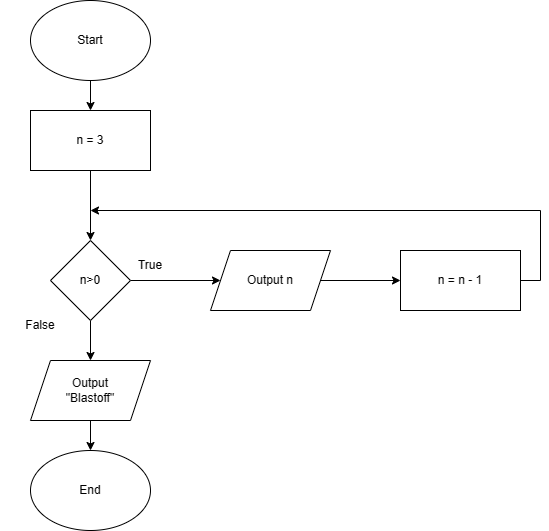
\includegraphics[width=9cm]{images/countdownwhileflow.png}
    \caption{Flowchart for the countdown program}
    \label{fig:countdownwhile}
\end{figure}
It is a little easier to understand how the code is looping by looking at the flowchart. Notice how after the n has one subtracted from it, the condition is checked again. That is the spot where it decides if the program will continue with the loop or end the loop.

More formally, the flow of execution for a {\tt while} statement
is as follows:

\begin{enumerate}

\item Evaluate the condition in parentheses, yielding {\tt true}
or {\tt false}.

\item If the condition is false, exit the {\tt while} statement
and continue execution at the next statement.

\item If the condition is true, execute each of the statements
between the curly-braces, and then go back to step 1.

\end{enumerate}

This type of flow is called a {\bf loop} because the third step loops
back around to the top.  Notice that if the condition is false the
first time through the loop, the statements inside the loop are
never executed.  The statements inside the loop are called
the {\bf body} of the loop.


\index{loop}
\index{loop!body}
\index{loop!infinite}
\index{body!loop}
\index{infinite loop}

The body of the loop should change the value of
one or more variables so that, eventually, the condition becomes
false and the loop terminates.  Otherwise the loop will repeat
forever, which is called an {\bf infinite loop}.  An endless
source of amusement for computer scientists is the observation
that the directions on shampoo, ``Lather, rinse, repeat,'' are
an infinite loop.

In the case of {\tt countdown}, we can prove that the loop
will terminate because we know that the value of {\tt n} is
finite, and we can see that the value of {\tt n} gets smaller
each time through the loop (each {\bf iteration}), so
eventually we have to get to zero.  In other cases it is not
so easy to tell:

\begin{verbatim}
    while (n != 1) {
      cout << n << endl;
      if (n%2 == 0) {           // n is even
        n = n / 2;
      } else {                  // n is odd
        n = n*3 + 1;
      }
    }

\end{verbatim}
%
The condition for this loop is {\tt n != 1}, so the loop
will continue until {\tt n} is 1, which will make the condition
false.

At each iteration, the program outputs the value of {\tt n} and then
checks whether it is even or odd.  If it is even, the value of
{\tt n} is divided by two.  If it is odd, the value is replaced
by $3n+1$.  For example, if the starting value (the argument passed
to {\tt sequence}) is 3, the resulting sequence is
3, 10, 5, 16, 8, 4, 2, 1.

Since {\tt n} sometimes increases and sometimes decreases, there is no
obvious proof that {\tt n} will ever reach 1, or that the program will
terminate.  For some particular values of {\tt n}, we can prove
termination.  For example, if the starting value is a power of two, then
the value of {\tt n} will be even every time through the loop, until
we get to 1.  The previous example ends with such a sequence,
starting with 16.

Particular values aside, the interesting question is whether
we can prove that this program terminates for {\em all} values of n.
So far, no one has been able to prove it {\em or} disprove it!

This book has a while loop simulator in order to help you understand while loops, \url{https://lpatacch.github.io/thinkCPPGamesEx/WhilePractice.html}. 
With this, you can change the 
initial value, the condition it is checking (\textless, \textgreater, ==, !=, \textgreater=, \textless=), the value checked,
and how the variable will change. Use this as many times as you wish
to understand how while loops work.
\section{New Operators}
Before we get more into loops, I want to cover some more math operators that we have not seen yet. In the countdown program, we had the counter change values with this equation:
\begin{verbatim}
    n = n-1;
\end{verbatim}
That equation took whatever was in n, subtracted 1, and placed it back in n. That behavior is very typical with loops. One variable 
is changed until it reaches the end value. It is so common that there is a short cut for this behavior. The above equation can be rewritten to this:
\begin{verbatim}
    n -= 1;
\end{verbatim}
This equation means the same as above, the value n has 1 subtracted from it, and then the result is put in n. Similar equations are available for many other math operators:
\begin{table}[h]
    \centering
    \begin{tabular}{|c|c|c|}
    \hline
 Math Operator & What it does & sample equation \\\hline
    +=     &  addition & {\tt n += 3;} \\
    -=      & subtraction & {\tt n -= 5;}\\
    {\tt *=}  &   multiplication & {\tt n *= 4;} \\
    \textbackslash=  &    division  & {\tt n \textbackslash= 2;}\\
    \%=  &  modulus & {\tt n \%= 7;}\\
\hline
    \end{tabular}
    \caption{New operators}
    \label{tab:newoperators}
\end{table}
\section{Increment and decrement operators}
\index{operator!increment}
\index{operator!decrement}

Incrementing and decrementing by one are such common operations that C++
provides special operators for them.  The {\tt ++} operator adds one
to the current value of an {\tt int}, {\tt char} or {\tt double}, and
{\tt --} subtracts one.  Neither operator works on {\tt string}s,
and neither {\em should} be used on {\tt bool}s.

The equation we modified in the last section:
\begin{verbatim}
    n -= 1;
\end{verbatim}

If you notice, the n was decremented by one. So, we can use the even shorter form here:
\begin{verbatim}
    --n;
\end{verbatim}
This subtracts 1 from n. This makes a very small line of code. All you need is the increment or the decrement operator, and the variable you will be changing.

You may have noticed that on some lines I put the ++ before the variable, and some after the variable. Both are legal. When it is on it's own line, it seems like it is doing the same thing. But, it is doing something slightly different. The ++ before the variable is called a pre-incrementor. It means that it will be doing the adding before anything else in the line. The ++ after the variable is called a post-incrementor. It means that it will be doing the adding after most of the things on the line. 

Technically, it is legal to increment a variable and use it
in an expression at the same time.  For example, you might see
something like:

\begin{verbatim}
  std::cout << i++ << std::endl;
\end{verbatim}
%
Looking at this, it is not clear whether the increment will
take effect before or after the value is displayed.  Because
expressions like this tend to be confusing, I would discourage
you from using them.  In fact, to discourage you even more,
I'm not going to tell you what the result is, other than letting you know it is a post-incrementor.  If you really
want to know, you can try it.

Using the increment operators, we can calculate the average weight of a person's inventory:

\begin{lstlisting}
  
  int num = 0;
  int weight = 0;
  int total = 0;
  std::cout << "Enter the weight of the item.\n"
  std::cout << "When done, enter -1\n";
  std::cin >> weight;
  while (weight >= 0) {
    //if it is a valid weight, add it to the total
    total += weight;
    
    //add one to the number of items
    ++num;
    
    //ask for the next weight
    std::cout << "Enter the weight of the item.\n"
    std::cout << "When done, enter -1\n";
    std::cin >> weight;    
  }
  
  if (num != 0)
  {
    std::cout << "The average is" << total/num <<".\n"; 
  }
  else {
    std::cout << "No items to average.\n";
  }
\end{lstlisting}
%
It is a common error to write something like

\begin{verbatim}
  num = num++;             // WRONG!!
\end{verbatim}
%
Unfortunately, this is syntactically legal, so the compiler
will not warn you.  The effect of this statement is to leave
the value of {\tt num} unchanged.  This is often a difficult
bug to track down.

Remember, you can write {\tt num = num +1;}, or you
can write {\tt num++;}, but you shouldn't mix them.

The ++ and -- does not work on a complex expression either. For example, 

\begin {verbatim}
( n + 7 )++;
\end{verbatim}
would not compile. The ++ and -- should be used only on a variable, not an expression.

\section{Parts of a loop}
The loops we have written so far have a number of elements
in common.  All of them start by initializing a variable;
they have a test, or condition, that depends on that variable;
and inside the loop they do something to that variable,
like increment it. This can be described by the following pseudocode:
\begin{verbatim}
  INITIALIZER;
  while (CONDITION) {
    BODY
    MODIFICATION
  }
\end{verbatim}
Loops, in order to work properly, need to have all three parts. If there is no modification section, the loop would never be able to leave the loop. If the initialization is wrong (or missing), the loop may loop the wrong amount of times (or never loop). And last, if the condition is wrong, the loop will never end properly. Whenever you loop is not working properly, if you look at those three parts, you will find the problem.

\section{Definite loop}
There are two different ways that loops can usually be identified. The first type 
is one where you know how many times the loop will repeat. These type of loops tend to
have a counter that is either counting down or up, and the counter is modified by a
constant value each time through the loop. These loops are sometimes called definite loops,
or counting loops. We have seen example with the countdown loop. The count down started at
three and the counter went down by one each time through the loop. Here is another example:

\begin{lstlisting}
  int val = 7;
  std::cout << "Here is a multiplication table for ";
  std::cout << val <<"\n";
  
  int x = 1;
  while (x <= 10)
  {
     std::cout << x << "\t" << x * val << "\n";
     x++;
  }
\end{lstlisting}
This loop has the condition as x<=10. If you look in the loop, you will notice that
x is being modified by 1 each time through the loop. Also, x is initialized to 1
when the loop starts. That means that the loop will repeat 10 times. Every time you
run this code, it will repeat 10 times.

In case you are interested, the \textbackslash t is one of the escape sequences that
we mentioned in \ref{tab:escapechar}. This spaces out each column by a tab stop. There 
are better ways to format tables, but we will not cover those methods for a while.

\section{Indefinite loop}
There is a different type of loop where you will not know how many times the loop
will run. The loop is checking a condition that will change, but it is different every
time we run the loop. We showed an example in the weight of the inventory code. This 
loop may have not repeated at all, or it could have repeated a thousand times. Since
you can not tell how many times it will repeat, it can be called an "indefinite loop". 
The number of repeats depended on what the user was entering. That code was waiting on a particular value (a negative number).
When a loop is waiting for a particular value, that value is called a flag, or a sentinel, which is why this loop may be
called a sentinel loop. 

FIXME: add an example

FIXME: code blocks
\section{{\tt do-while} loop}
The second type of loop that C++ supports is called a do-while loop.
It works very similarly to the while loop. It should be initialized
before the loop starts, it should be modified inside the loop, and
it has a condition it checks. The difference is where it checks the
condition. The do-while loop checks the condition at the end of the
loop, guaranteeing the loop always runs at least once. The while loop
checks the condition at the beginning, which could mean the loop
might not run at all. The general syntax looks like the following:

\begin{verbatim}
  INITIALIZER;
   do {
    BODY
    MODIFICATION
  } while (CONDITION);
\end{verbatim}
%

For example, the multiplication table could be changed to a do-while:
\begin{lstlisting}
  int val = 7;
  std::cout << "Here is a multiplication table for ";
  std::cout << val <<"\n";
  
  int x = 1;
  do {
     std::cout << x << "\t" << x * val << "\n";
     x++;
  } while (x <= 10);
\end{lstlisting}
\begin{figure}[h]
    \centering
    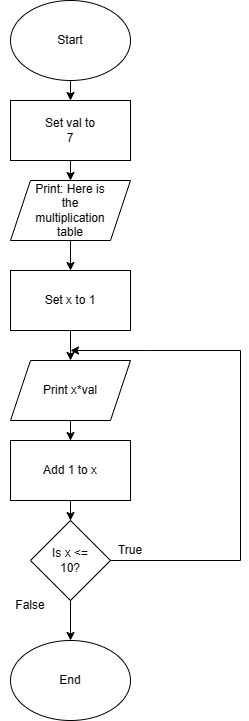
\includegraphics[height=10cm]{images/do-whileflow.png}
    \caption{Flowchart for the do-while multiplication table}
    \label{fig:do-while}
\end{figure}
By now, you may be wondering, "Why should I use this approach instead of a while loop?" The main advantage is that the code within the loop is guaranteed to execute at least once. I often use this type of loop when obtaining input from the user. In many programs, we ask a question. Unfortunately, the user may not always provide a valid response. While we know that we need to ask the question once, we cannot be certain if we will need to repeat it if the user provides an incorrect response. For instance, let's consider an example where we ask the user whether they want to turn left or right. The only correct answer is 'l' or 'r'. \footnote{Technically, we should have changed the answer to lowercase to allow for L and R,
but I wanted this example to be simpler than that.}
\begin{lstlisting}
  char direction = '\0';
  do {
     std::cout << "Do you want to go (l)eft or (r)ight?\n");
     std::cin >> direction;
     if ((direction != 'l')&&(direction != 'r'))
     {
        std::cout << "Please enter l or r\n";
     }
  } while ((direction != 'l')&&(direction != 'r'));
\end{lstlisting}
If we decided to do this with a while, we would have needed to ask 
the question both outside and inside the loop. This reduces the 
amount of times the same code is written in the program.

\section{{\tt for} loops}
\index{loop!for}
\index{for}
\index{statement!for}
We have had many examples of definite or counting loops.
This type of loop is so common that there is an alternate
loop statement, called {\tt for}, that expresses it more
concisely.  The general syntax looks like this:

\begin{verbatim}
  for (INITIALIZER; CONDITION; INCREMENTOR) {
    BODY
  }
\end{verbatim}
%
This statement is exactly equivalent to

\begin{verbatim}
  INITIALIZER;
  while (CONDITION) {
    BODY
    INCREMENTOR
  }
\end{verbatim}
%
except that it is more concise and, since it puts all the
loop-related statements in one place, it is easier to read.
For example:

\begin{verbatim}
  int i;
  for (i = 0; i < 4; i++) {
    cout << i << endl;
  }
\end{verbatim}
%
is equivalent to 

\begin{verbatim}
  int i = 0;
  while (i < 4) {
    cout << i << endl;
    i++;
  }
\end{verbatim}

FIXME - example of for loop with a decrement instead
FIXME - example of for loop with a step of 5

\section{Break and Continue}
FIXME add examples of how this works
\section{Glossary}

\begin{description}

\item[loop:]  A statement that executes repeatedly while a
condition is true or until some condition is satisfied.

\item[infinite loop:]  A loop whose condition is always true.

\item[body:]  The statements inside the loop.

\item[iteration:]  One pass through (execution of) the body
of the loop, including the evaluation of the condition.


\index{loop}
\index{infinite loop}
\index{body}
\index{loop!infinite}
\index{iteration}


\end{description}


% LaTeX source for textbook ``ThinkCPP , a game perspective''
% Copyright (C) 2023  Lisa Patacchiola 

\chapter{Game Loops}
FIXME - put the game loop information here
% LaTeX source for textbook ``ThinkCPP , a game perspective''
% Copyright (C) 2023 Lisa Patacchiola, Allen B. Downey

\chapter{Function}

\section{Math functions}
\index{math function}
\index{function!Math}
\index{expression}
\index{argument}
\label{mathlibrary}

In mathematics, you have probably seen functions like $\sin$ and
$\log$, and you have learned to evaluate expressions like
$\sin(\pi/2)$ and $\log(1/x)$.  First, you evaluate the
expression in parentheses, which is called the {\bf argument} of the
function.  For example, $\pi/2$ is approximately 1.571, and $1/x$ is
0.1 (if $x$ happens to be 10).

Then you can evaluate the function itself, either by looking it up in
a table or by performing various computations.  The $\sin$ of 1.571 is
1, and the $\log$ of 0.1 is -1 (assuming that $\log$ indicates the
logarithm base 10).

This process can be applied repeatedly to evaluate more complicated
expressions like $\log(1/\sin(\pi/2))$.  First we evaluate the
argument of the innermost function, then evaluate the function,
and so on.

C++ provides a set of built-in functions that includes most
of the mathematical operations you can think of.
The math functions are invoked using a syntax that is similar to
mathematical notation:

\begin{verbatim}
     double log = std::log (17.0);
     double angle = 1.5;
     double height = std::sin (angle);
\end{verbatim}
%
The first example sets {\tt log} to the logarithm of 17, base
$e$.  There is also a function called {\tt log10} that takes
logarithms base 10.

The second example finds the sine of the value of the variable
{\tt angle}.  C++ assumes that the
values you use with {\tt sin} and the other trigonometric functions
({\tt cos}, {\tt tan}) are in {\em radians}.  To
convert from degrees to radians, you can divide by 360
and multiply by $2 \pi$.  

If you don't happen to know $\pi$ to 15 digits, you can
calculate it using the {\tt acos} function.  The arccosine
(or inverse cosine) of -1 is $\pi$, because the cosine of
$\pi$ is -1.

\begin{verbatim}
  double pi = std::acos(-1.0);
  double degrees = 90;
  double angle = degrees * 2 * pi / 360.0;
\end{verbatim}
%
Before you can use any of the math functions, you have to
include the cmath {\bf header file}.  Header files contain
information the compiler needs about functions that are defined
outside your program.  For example, in the ``Hello, world!''
program we included a header file named {\tt iostream} using
an {\bf include} statement:

\begin{verbatim}
#include <iostream>
using namespace std;
\end{verbatim}
%
{\tt iostream} contains information about input and output
(I/O) streams, including the object named {\tt cout}.
C++ has a powerful feature called namespaces, that
allow you to write your own implementation of {\tt cout}.
But in most cases, we would need to use the standard implementation.
To convey this to the compiler, we use the line

\begin{verbatim}
using namespace std;
\end{verbatim}

To save yourself some typing, you can write {\tt using namespace std;} whenever
you use {\tt iostream}. This allows a shorthand where you can skip
typing the std:: in your code. For example, the hello world program
could be shortened to the following:
\begin{lstlisting}
#include <iostream>
using namespace std;

// main: generate some simple output
int main ()
{
  cout << "Hello, world." << endl;
  return 0;
}
\end{lstlisting}
%
However, in general it is not good practice, since it imports the 
entirety of std into your program.  This can become a problem when your programs get 
more complicated, and it takes over some of the namespace you would
want to use.
For this course it is an acceptable time-saving device, but I would
suggest you remove it for any portfolio projects. 

\index{header file}
\index{cmath}
\index{iostream}

Just like iostream, the math header file contains information
about the math functions.  You can include it at the beginning
of your program along with {\tt iostream}:

\begin{verbatim}
#include <cmath>
\end{verbatim}

Such header files have an initial `c' to signify that these
header files have been derived from the {\bf C} language.
\section{Math constants}
Although you can calculate PI using acos, C++ has done the calculation
ahead of time for you. If you are using C++20 or later, you can use the values in std::numbers. 

\begin{verbatim}
double mypi = std::numbers::pi;
\end{verbatim}
There are many other values available too, like e and phi.

If you are using an older version of the compilers, you may need to 
use a different technique to get PI. If you are including <cmath>, you should also have M\_PI defined.

\begin{verbatim}
double mypi = M_PI;
\end{verbatim}

If you have a very old version of C++, it may need a special line above the include cmath in order for M\_PI to work. But, I suggest you try the above versions
first before using this:

\begin{verbatim}
#define _USE_MATH_DEFINES
#include <cmath>
\end{verbatim}

\section {Composition}
\label{composition}
\index{composition}
\index{expression}

Just as with mathematical functions, C++ functions can be {\bf
composed}, meaning that you use one expression as part of another.
For example, you can use any expression as an argument to a function:

\begin{verbatim}
    double x = cos (angle + pi/2);
\end{verbatim}
%
This statement takes the value of {\tt pi}, divides it by two and
adds the result to the value of {\tt angle}.  The sum is
then passed as an argument to the {\tt cos} function.

You can also take the result of one function and pass it as
an argument to another:

\begin{verbatim}
    double x = exp (log (10.0));
\end{verbatim}
%
This
statement finds the log base $e$ of 10 and then raises $e$ to that
power.  The result gets assigned to {\tt x}; I hope you know what it
is.

\section{Adding new functions}
\index{function!definition}
\index{main}
\index{function!main}

So far we have only been using the functions that are built into C++,
but it is also possible to add new functions.  Actually, we have already
seen one function definition: {\tt main}.  The function named {\tt main}
is special because it indicates where the execution of the program
begins, but the syntax for {\tt main} is the same as for any other
function definition:

\begin{verbatim}
  void NAME ( LIST OF PARAMETERS ) {
    STATEMENTS
  }
\end{verbatim}
%
You can make up any name you want for your function, except
that you can't call it {\tt main} or any other
C++ keyword.  The list of
parameters specifies what information, if any, you have to
provide in order to use (or {\bf call}) the new function.

{\tt main} doesn't take any parameters, as indicated by
the empty parentheses {\tt ()} in it's definition\footnote{You can add parameters in main to get access to the command line parameters. We will show how to use them much later in the book. For now, it is OK to use main without parameters. }.  The first couple
of functions we are going to write also have no parameters, so the
syntax looks like this:

\begin{verbatim}
  void newLine () {
    std::cout << std::endl;
  }
\end{verbatim}
%
This function is named {\tt newLine}; it contains only a single
statement, which outputs a newline character, represented by
the special value {\tt endl}.

In {\tt main} we can call this new function using syntax that
is similar to the way we call the built-in C++ commands:

\begin{verbatim}
int main ()
{
  std::cout << "First Line." << std::endl;
  newLine ();
  std::cout << "Second Line." << std::endl;
  return 0;
}
\end{verbatim}
%
The output of this program is

\begin{verbatim}
First line.

Second line.
\end{verbatim}
%
Notice the extra space between the two lines.  What if we wanted
more space between the lines?  We could call the same
function repeatedly:

\begin{verbatim}
int main ()
{
  std::cout << "First Line." << std::endl;
  newLine ();
  newLine ();
  newLine ();
  std::cout << "Second Line." << std::endl;
  return 0;
}
\end{verbatim}
%

We could use a for loop to call it multiple times:
\begin{verbatim}
int main ()
{
  std::cout << "First Line." << std::endl;
  for (int x = 0; x < 3; x++) {
     newLine ();
  }
  std::cout << "Second Line." << std::endl;
  return 0;
}
\end{verbatim}
It is acceptable to have a function inside a loop. 
Or we could write a new function, named {\tt threeLine}, that 
prints three new lines:

\begin{verbatim}
void threeLine ()
{
  newLine ();  newLine ();  newLine ();
}

int main ()
{
  std::cout << "First Line." << std::endl;
  threeLine ();
  std::cout << "Second Line." << std::endl;
  return 0;
}
\end{verbatim}
%
You should notice a few things about this program:

\begin{itemize}

\item You can call the same procedure repeatedly.  In
fact, it is quite common and useful to do so.

\item You can have one function call another function.  In this
case, {\tt main} calls {\tt threeLine} and {\tt threeLine}
calls {\tt newLine}.  Again, this is common and useful.

\item In {\tt threeLine} I wrote three statements all on the
same line, which is syntactically legal (remember that spaces
and new lines usually don't change the meaning of a program).
On the other hand, it is usually a better idea to put each
statement on a line by itself, to make your program easy to
read.  I sometimes break that rule in this book to save space.

\end{itemize}

So far, it may not be clear why it is worth the trouble to
create all these new functions.  Actually, there are a lot
of reasons, but this example only demonstrates two:

\begin{enumerate}

\item Creating a new function gives you an opportunity to
give a name to a group of statements.  Functions can simplify a program
by hiding a complex computation behind a single command, and by using
English words in place of arcane code.  Which is clearer, {\tt
newLine} or {\tt cout << endl}?

\item Creating a new function can make a program smaller by eliminating
repetitive code.  For example, a short way to print nine consecutive
new lines is to call {\tt threeLine} three times.  How would you
print 27 new lines?

\end{enumerate}

\section {Definitions and uses}

Pulling together all the code fragments from the previous
section, the whole program looks like this:

\begin{verbatim}
#include <iostream>
using namespace std;

void newLine ()
{
  cout << endl;
}

void threeLine ()
{
  newLine ();  newLine ();  newLine ();
}

int main ()
{
  cout << "First Line." << endl;
  threeLine ();
  cout << "Second Line." << endl;
  return 0;
}
\end{verbatim}

This program contains three function definitions: {\tt newLine},
{\tt threeLine}, and {\tt main}.

Inside the definition of {\tt main}, there is a statement that
uses or calls {\tt threeLine}.  Similarly, {\tt threeLine} calls
{\tt newLine} three times.  Notice that the definition of each
function appears above the place where it is used.

This is necessary in C++; the definition of a function must
appear before (above) the first use of the function.  You
should try compiling this program with the functions in a
different order and see what error messages you get.

\section {Programs with multiple functions}

When you look at a class definition that contains several functions, it
is tempting to read it from top to bottom, but that is likely to be
confusing, because that is not the {\bf order of execution} of the
program.

Execution always begins at the first statement of {\tt main},
regardless of where it is in the program (often it is at the bottom).
Statements are executed one at a time, in order, until you reach a
function call.  Function calls are like a detour in the flow of
execution.  Instead of going to the next statement, you go to the
first line of the called function, execute all the statements there,
and then come back and pick up again where you left off.

That sounds simple enough, except that you have to remember that one
function can call another.  Thus, while we are in the middle of {\tt
main}, we might have to go off and execute the statements in {\tt
threeLine}.  But while we are executing {\tt threeLine}, we get
interrupted three times to go off and execute {\tt newLine}.

Fortunately, C++ is adept at keeping track of where it is, so
each time {\tt newLine} completes, the program picks up where it left
off in {\tt threeLine}, and eventually gets back to {\tt main} so the
program can terminate.

What's the moral of this sordid tale?  When you read a program, don't
read from top to bottom.  Instead, follow the flow of execution.

\section {Parameters and arguments}
\index{parameter}
\index{argument}

Some of the built-in functions we have used have {\bf parameters},
which are values that you provide to let the function do its
job.  For example, if you want to find the sine of a number,
you have to indicate what the number is.  Thus, {\tt sin}
takes a {\tt double} value as a parameter.

Some functions take more than one parameter, like {\tt pow},
which takes two {\tt doubles}, the base and the exponent.

Notice that in each of these cases we have to specify not
only how many parameters there are, but also what type they
are.  So it shouldn't surprise you that when you write a
class definition, the parameter list indicates the type of
each parameter.  For example:

\begin{verbatim}
  void printTwice (char phil) {
    cout << phil << phil << endl;
  }
\end{verbatim}
%
This function takes a single parameter, named {\tt phil}, that
has type {\tt char}.  Whatever that parameter is (and at
this point we have no idea what it is), it gets printed
twice, followed by a newline.
I chose the name {\tt phil} to suggest that the name
you give a parameter is up to you, but in general you want to
choose something more illustrative than {\tt phil}.

In order to call this function, we have to provide a {\tt char}.
For example, we might have a {\tt main} function like this:

\begin{verbatim}
  int main () {
    printTwice ('a');
    return 0;
  }
\end{verbatim}
%
The {\tt char} value you provide is called an {\bf argument}, and we
say that the argument is {\bf passed} to the function.  In this
case the value {\tt 'a'} is passed as an argument
to {\tt printTwice} where it will get printed twice.

Alternatively, if we had a {\tt char} variable, we could
use it as an argument instead:

\begin{verbatim}
  int main () {
    char argument = 'b';
    printTwice (argument);
    return 0;
  }
\end{verbatim}
%
Notice something very important here: the name of the variable we pass
as an argument ({\tt argument}) has nothing to do with the name of the
parameter ({\tt phil}).  Let me say that again:

\begin{quote}

{\bf The name of the variable we pass as an argument has nothing to do
with the name of the parameter.}

\end{quote}

They can be the same or they can be different, but it is important
to realize that they are not the same thing, except that they happen
to have the same value (in this case the character {\tt 'b'}).

The value you provide as an argument must have the same type as
the parameter of the function you call.  This rule is
important, but it is sometimes confusing because C++ sometimes
converts arguments from one type to another automatically.  For
now you should learn the general rule, and we will deal with
exceptions later.

\section {Parameters and variables are local}

Parameters and
variables only exist inside their own functions.  Within the
confines of {\tt main}, there is no such thing as {\tt phil}.
If you try to use it, the compiler will complain.  Similarly,
inside {\tt printTwice} there is no such thing as {\tt argument}.

Variables like this are said to be {\bf local}.  In order to
keep track of parameters and local variables, it is useful to
draw a {\bf stack diagram}.  Like state diagrams, stack diagrams
show the value of each variable, but the variables are contained
in larger boxes that indicate which function they belong to.

For example, the stack diagram for {\tt printTwice} looks like this in figure \ref{fig:stack}:

\vspace{0.1in}
\begin{figure}[h]
    \centering
    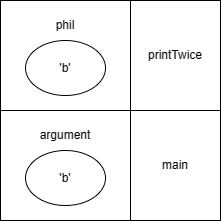
\includegraphics[height=6cm]{images/stack.png}
    \caption{Stack diagram from when printTwice is called}
    \label{fig:stack}
\end{figure}
%
Whenever a function is called, it creates a new {\bf instance}
of that function.  Each instance of a function contains the
parameters and local variables for that function.  In the
diagram an instance of a function is represented by a box
with the name of the function on the outside and the variables
and parameters inside.

In the example, {\tt main} has one local variable, {\tt argument}, and
no parameters.  {\tt printTwice} has no local variables and one
parameter, named {\tt phil}.

\section {Functions with multiple parameters}
\index{parameter!multiple}
\index{function!multiple parameter}
\index{class!Time}

The syntax for declaring and invoking functions with multiple
parameters is a common source of errors.  First, remember
that you have to declare the type of every parameter.  For
example

\begin{verbatim}
  void printTime (int hour, int minute) {
    cout << hour;
    cout << ":";
    cout << minute;
  }
\end{verbatim}
%
It might be tempting to write {\tt (int hour, minute)}, but
that format is only legal for variable declarations, not
for parameters.

Another common source of confusion is that you do not have
to declare the types of arguments.  The following is wrong!

\begin{verbatim}
    int hour = 11;
    int minute = 59;
    printTime (int hour, int minute);   // WRONG!
\end{verbatim}
%
In this case, the compiler can tell the type of {\tt hour}
and {\tt minute} by looking at their declarations.  It is
unnecessary and illegal to include the type when you pass them
as arguments.  The correct
syntax is {\tt printTime (hour, minute)}.

\label{printparity}
Do you remember the if/else code we did in the Chapter \ref{alternative} to check if something was even or odd? If you think you might want to check the parity
(evenness or oddness) of numbers often, you might want to
``wrap'' this code up in a function, as follows:

\begin{lstlisting}

void printParity (int x) {
  if (x%2 == 0) {
    std::cout << "x is even" << std::endl;
  } else {
    std::cout << "x is odd" << std::endl;
  }
}
\end{lstlisting}
%
Now you have a function named {\tt printParity} that will display
an appropriate message for any integer you care to provide. It is perfectly acceptable to have an if statement in a function.
In {\tt main} you would call this function as follows:

\begin{verbatim}
    printParity (17);
\end{verbatim}
%
Always remember that when you {\em call} a function, you do
not have to declare the types of the arguments you provide.
C++ can figure out what type they are.  You should resist the
temptation to write things like:

\begin{verbatim}
  int number = 17;
  printParity (int number);         // WRONG!!!
\end{verbatim}
\section {Functions with results}
\index{fruitful function}
\index{function!fruitful}

You might have noticed by now that some of the functions we are using,
like the math functions, yield results.  Other functions,
like {\tt newLine}, perform an action but
don't return a value.  That raises some questions:

\begin{itemize}

\item What happens if you call a function and you don't
do anything with the result (i.e. you don't assign it to
a variable or use it as part of a larger expression)?

\item What happens if you use a function without a result as part
of an expression, like {\tt newLine() + 7}?

\item Can we write functions that yield results, or are we
stuck with things like {\tt newLine} and {\tt printTwice}?

\end{itemize}

The answer to the third question is ``yes, you can write functions that
return values,'' and we'll do it in Chapter~\ref{fruitful functions}.  I will
leave it up to you to answer the other two questions by trying them
out.  Any time you have a question about what is legal or
illegal in C++, a good way to find out is to ask the compiler.

\section{The {\tt return} statement}
\index{return}
\index{statement!return}

The {\tt return} statement allows you to terminate the execution
of a function before you reach the end.  One reason to use it
is if you detect an error condition:

\begin{verbatim}
#include <cmath>

void printLogarithm (double x) {
  if (x <= 0.0) {
    cout << "Positive numbers only, please." << endl;
    return;
  }

  double result = log (x);
  cout << "The log of x is " << result;
}
\end{verbatim}
%
This defines a function named {\tt printLogarithm} that takes
a {\tt double} named {\tt x} as a parameter.  The first thing
it does is check whether {\tt x} is less than or equal to
zero, in which case it displays an error message and then uses
{\tt return} to exit the function.  The flow of execution
immediately returns to the caller and the remaining lines of
the function are not executed.

I used a floating-point value on the right side of the condition
because there is a floating-point variable on the left.

Remember that any time you want to use one a function from the math
library, you have to include the header file {\tt cmath}.

\section{Recursion}
\label{recursion}
\index{recursion}

I mentioned in the last chapter that it is legal for one function to
call another, and we have seen several examples of that.  I neglected
to mention that it is also legal for a function to call itself.  It
may not be obvious why that is a good thing, but it turns out to be
one of the most magical and interesting things a program can do.

For example, look at the following function:

\begin{verbatim}
void countdown (int n) {
  if (n == 0) {
    cout << "Blastoff!" << endl;
  } else {
    cout << n << endl;
    countdown (n-1);
  }
}
\end{verbatim}
%
The name of the function is {\tt countdown} and it takes a single
integer as a parameter.  If the parameter is zero, it outputs
the word ``Blastoff.''  Otherwise, it outputs the parameter and
then calls a function named {\tt countdown}---itself---passing
{\tt n-1} as an argument.

What happens if we call this function like this:

\begin{verbatim}
#include <iostream>
#include <cmath>
using namespace std;
void printLogarithm (double x) {
  if (x <= 0.0) {
    cout << "Positive numbers only, please." << endl;
    return;
  }

  double result = log (x);
  cout << "The log of x is " << result;
}

void countdown (int n) {
  if (n == 0) {
    cout << "Blastoff!" << endl;
  } else {
    cout << n << endl;
    countdown (n-1);
  }
}

int main ()
{
  countdown (3);
  return 0;
}
\end{verbatim}
%
The execution of {\tt countdown} begins with {\tt n=3}, and
since {\tt n} is not zero, it outputs the value 3, and then
calls itself...

\begin{quote}
The execution of {\tt countdown} begins with {\tt n=2}, and
since {\tt n} is not zero, it outputs the value 2, and then
calls itself...

\begin{quote}
The execution of {\tt countdown} begins with {\tt n=1}, and
since {\tt n} is not zero, it outputs the value 1, and then
calls itself...

\begin{quote}
The execution of {\tt countdown} begins with {\tt n=0}, and
since {\tt n} is zero, it outputs the word ``Blastoff!''
and then returns.
\end{quote}

The countdown that got {\tt n=1} returns.

\end{quote}

The countdown that got {\tt n=2} returns.

\end{quote}

The countdown that got {\tt n=3} returns.

\noindent And then you're back in {\tt main} (what a trip).  So the
total output looks like:

\begin{verbatim}
3
2
1
Blastoff!
\end{verbatim}
%
As a second example, let's look again at the functions
{\tt newLine} and {\tt threeLine}.

\begin{verbatim}
void newLine () {
  cout << endl;
}

void threeLine () {
  newLine ();  newLine ();  newLine ();
}
\end{verbatim}
%
Although these work, they would not be much help if I wanted
to output 2 newlines, or 106.  A better alternative would be

\begin{verbatim}
void nLines (int n) {
  if (n > 0) {
    cout << endl;
    nLines (n-1);
  }
}
\end{verbatim}
%
This program is similar to {\tt countdown}; as long as {\tt n} is
greater than zero, it outputs one newline, and then calls itself to
output {\tt n-1} additional newlines.  Thus, the total number of
newlines is {\tt 1 + (n-1)}, which usually comes out to roughly {\tt
n}.

\index{recursive}
\index{newline}

The process of a function calling itself is called {\bf recursion}, and
such functions are said to be {\bf recursive}.

\section {Infinite recursion}

In the examples in the previous section, notice that each time the
functions get called recursively, the argument gets smaller by one, so
eventually it gets to zero.  When the argument is zero, the function
returns immediately, {\em without making any recursive calls}.
This case---when the function completes without making a recursive
call---is called the {\bf base case}.

If a recursion never reaches a base case, it will go on making recursive
calls forever and the program will never terminate.  This is known as
{\bf infinite recursion}, and it is generally not considered a good
idea.

\index{recursion!infinite}
\index{infinite recursion}
\index{run-time error}

In most programming environments, a program with an infinite
recursion will not really run forever.  Eventually, something
will break and the program will report an error.  This is the
first example we have seen of a run-time error (an error that
does not appear until you run the program).

You should write a small program that recurses forever and run
it to see what happens.

\section {Stack diagrams for recursive functions}
\index{stack}
\index{diagram!state}
\index{diagram!stack}

In a previous section we used a stack diagram to represent the
state of a program during a function call.  The same kind
of diagram can make it easier to interpret a recursive function.

Remember that every time a function gets called it creates
a new instance that contains
the function's local variables and parameters.

This figure shows a stack diagram for countdown, called
with {\tt n = 3}:

\vspace{0.1in}
\centerline{\epsfig{figure=oldimages/stack2.eps}}
\vspace{0.1in}
%
There is one instance of {\tt main} and four instances of
{\tt countdown}, each with a different value for the parameter
{\tt n}.  The bottom of the stack, {\tt countdown} with {\tt n=0}
is the base case.  It does not make a recursive call, so there
are no more instances of {\tt countdown}.

The instance of {\tt main} is empty because {\tt main} does not
have any parameters or local variables.  As an exercise, draw a
stack diagram for {\tt nLines}, invoked with the parameter {\tt n=4}.



\section{Glossary}

\begin{description}

\item[initialization:]  A statement that declares a new variable
and assigns a value to it at the same time.

\item[function:]  A named sequence of statements that performs some
useful function.  Functions may or may not take parameters, and may
or may not produce a result.

\item[parameter:]  A piece of information you provide
in order to call a function.  Parameters are like variables in
the sense that they contain values and have types.

\item[argument:]  A value that you provide when you call a
function.  This value must have the same type as the corresponding
parameter.

\item[call:]  Cause a function to be executed.

\item[recursion:]  The process of calling the same function you
are currently executing.

\item[infinite recursion:]  A function that calls itself
recursively without every reaching the base case.  Eventually
an infinite recursion will cause a run-time error.

\index{function}
\index{parameter}
\index{argument}
\index{call}
\index{initialization}
\index{recursion}
\index{recursion!infinite}
\index{infinite recursion}

\end{description}


% LaTeX source for textbook ``How to think like a computer scientist''
% Copyright (C) 1999  Allen B. Downey



\chapter{Iteration}

\section{Multiple assignment}
\index{assignment}
\index{statement!assignment}
\index{multiple assignment}

I haven't said much about it, but it is legal in C++ to
make more than one assignment to the same variable.  The
effect of the second assignment is to replace the old value
of the variable with a new value.

\begin{verbatim}
  int fred = 5;
  cout << fred;
  fred = 7;
  cout << fred;
\end{verbatim}
%
The output of this program is {\tt 57}, because the first
time we print {\tt fred} his value is 5, and the second time
his value is 7.

This kind of {\bf multiple assignment} is the reason I
described variables as a {\em container} for values.  When
you assign a value to a variable, you change the contents of
the container, as shown in the figure:

\vspace{0.1in}
\centerline{\epsfig{figure=assign2.eps}}
\vspace{0.1in}

When there are multiple assignments to a variable, it is especially
important to distinguish between an assignment statement and a
statement of equality.  Because C++ uses the {\tt =} symbol for
assignment, it is tempting to interpret a statement like {\tt a = b}
as a statement of equality.  It is not!

First of all, equality is commutative, and assignment is not.
For example, in mathematics if $a = 7$ then $7 = a$.  But in
C++ the statement {\tt a = 7;} is legal, and {\tt 7 = a;}
is not.

Furthermore, in mathematics, a statement of equality is true
for all time.  If $a = b$ now, then $a$ will always equal $b$.
In C++, an assignment statement can make two variables equal,
but they don't have to stay that way!

\begin{verbatim}
  int a = 5;
  int b = a;     // a and b are now equal
  a = 3;         // a and b are no longer equal
\end{verbatim}
%
The third line changes the value of {\tt a} but it does not
change the value of {\tt b}, and so they are no longer equal.
In many programming languages an alternate symbol is used
for assignment, such as {\tt <-} or {\tt :=}, in order to
avoid confusion.

Although multiple assignment is frequently useful, you should
use it with caution.  If the values of variables are changing
constantly in different parts of the program, it can make
the code difficult to read and debug.

\section{Iteration}
\index{iteration}

One of the things computers are often used for is the automation
of repetitive tasks.  Repeating identical or similar tasks without
making errors is something that computers do well and people do
poorly.

We have seen programs that use recursion to perform
repetition, such as {\tt nLines} and {\tt countdown}.  This
type of repetition is called {\bf iteration}, and C++ provides
several language features that make it easier to write iterative
programs.

The two features we are going to look at are the {\tt while}
statement and the {\tt for} statement.

\section{The {\tt while} statement}
\index{statement!while}
\index{while statement}

Using a {\tt while} statement, we can rewrite {\tt countdown}:

\begin{verbatim}
int countdown (int n) {
  while (n > 0) {
    cout << n << endl;
    n = n-1;
  }
  cout << "Blastoff!" << endl;
  return 0;
}
\end{verbatim}
%
You can almost read a {\tt while} statement as if it were
English.  What this means is, ``While {\tt n} is greater than
zero, continue displaying the value of {\tt n} and then reducing
the value of {\tt n} by 1.  When you get to zero, output the
word `Blastoff!'''

More formally, the flow of execution for a {\tt while} statement
is as follows:

\begin{enumerate}

\item Evaluate the condition in parentheses, yielding {\tt true}
or {\tt false}.

\item If the condition is false, exit the {\tt while} statement
and continue execution at the next statement.

\item If the condition is true, execute each of the statements
between the squiggly-braces, and then go back to step 1.

\end{enumerate}

This type of flow is called a {\bf loop} because the third step loops
back around to the top.  Notice that if the condition is false the
first time through the loop, the statements inside the loop are
never executed.  The statements inside the loop are called
the {\bf body} of the loop.

\index{loop}
\index{loop!body}
\index{loop!infinite}
\index{body!loop}
\index{infinite loop}

The body of the loop should change the value of
one or more variables so that, eventually, the condition becomes
false and the loop terminates.  Otherwise the loop will repeat
forever, which is called an {\bf infinite loop}.  An endless
source of amusement for computer scientists is the observation
that the directions on shampoo, ``Lather, rinse, repeat,'' are
an infinite loop.

In the case of {\tt countdown}, we can prove that the loop
will terminate because we know that the value of {\tt n} is
finite, and we can see that the value of {\tt n} gets smaller
each time through the loop (each {\bf iteration}), so
eventually we have to get to zero.  In other cases it is not
so easy to tell:

\begin{verbatim}
  void sequence (int n) {
    while (n != 1) {
      cout << n << endl;
      if (n%2 == 0) {           // n is even
        n = n / 2;
      } else {                  // n is odd
        n = n*3 + 1;
      }
    }
  }
\end{verbatim}
%
The condition for this loop is {\tt n != 1}, so the loop
will continue until {\tt n} is 1, which will make the condition
false.

At each iteration, the program outputs the value of {\tt n} and then
checks whether it is even or odd.  If it is even, the value of
{\tt n} is divided by two.  If it is odd, the value is replaced
by $3n+1$.  For example, if the starting value (the argument passed
to {\tt sequence}) is 3, the resulting sequence is
3, 10, 5, 16, 8, 4, 2, 1.

Since {\tt n} sometimes increases and sometimes decreases, there is no
obvious proof that {\tt n} will ever reach 1, or that the program will
terminate.  For some particular values of {\tt n}, we can prove
termination.  For example, if the starting value is a power of two, then
the value of {\tt n} will be even every time through the loop, until
we get to 1.  The previous example ends with such a sequence,
starting with 16.

Particular values aside, the interesting question is whether
we can prove that this program terminates for {\em all} values of n.
So far, no one has been able to prove it {\em or} disprove it!

\section{Definite loop}
count example
\section{indefinite loop}
sentinel example
\section{Tables}
\index{table}
\index{logarithm}

One of the things loops are good for is generating
tabular data.  For example, before computers were readily available,
people had to calculate logarithms, sines and cosines, and other
common mathematical functions by hand.
To make that easier, there were books containing long tables
where you could find the values of various functions.
Creating these tables was slow and boring, and the result
tended to be full of errors.

When computers appeared on the scene, one of the initial reactions
was, ``This is great!  We can use the computers to generate the
tables, so there will be no errors.''  That turned out to be true
(mostly), but shortsighted.  Soon thereafter computers and
calculators were so pervasive that the tables became obsolete.

Well, almost.  It turns out that for some operations, computers
use tables of values to get an approximate answer, and then
perform computations to improve the approximation.  In some
cases, there have been errors in the underlying tables, most
famously in the table the original Intel Pentium used to perform
floating-point division.

\index{division!floating-point}

Although a ``log table'' is not as useful as it once was, it still
makes a good example of iteration.  The following program outputs a
sequence of values in the left column and their logarithms in the
right column:

\begin{verbatim}
  double x = 1.0;
  while (x < 10.0) {
    cout << x << "\t" << log(x) << "\n";
    x = x + 1.0;
  }
\end{verbatim}
%
The sequence \verb+\t+ represents a {\bf tab} character.
The
sequence \verb+\n+ represents a newline character.  These sequences
can be included anywhere in a string, although in these examples
the sequence is the whole string.

A tab character causes the cursor to shift to the right until
it reaches one of the {\bf tab stops}, which are normally every
eight characters.  As we will see in a minute, tabs are useful
for making columns of text line up.

A newline character has exactly the same effect as {\tt endl};
it causes the cursor to move on to the next line.  Usually if
a newline character appears by itself, I use {\tt endl}, but
if it appears as part of a string, I use \verb+\n+.

The output of this program is

\begin{verbatim}
1      0
2      0.693147
3      1.09861
4      1.38629
5      1.60944
6      1.79176
7      1.94591
8      2.07944
9      2.19722
\end{verbatim}
%
If these values seem odd, remember that the {\tt log} function uses
base $e$.  Since powers of two are so important in computer science,
we often want to find logarithms with respect to base 2.  To do that,
we can use the following formula:

\[ \log_2 x = \frac {log_e x}{log_e 2} \]
%
Changing the output statement to

\begin{verbatim}
      cout << x << "\t" << log(x) / log(2.0) << endl;
\end{verbatim}
%
yields

\begin{verbatim}
1      0
2      1
3      1.58496
4      2
5      2.32193
6      2.58496
7      2.80735
8      3
9      3.16993
\end{verbatim}
%
We can see that 1, 2, 4 and 8 are powers of two, because
their logarithms base 2 are round numbers.  If we wanted to find
the logarithms of other powers of two, we could modify the
program like this:

\begin{verbatim}
  double x = 1.0;
  while (x < 100.0) {
    cout << x << "\t" << log(x) / log(2.0) << endl;
    x = x * 2.0;
  }
\end{verbatim}
%
Now instead of adding something to {\tt x} each time through
the loop, which yields an arithmetic sequence, we multiply
{\tt x} by something, yielding a {\bf geometric} sequence.
The result is:

\begin{verbatim}
1      0
2      1
4      2
8      3
16     4
32     5
64     6
\end{verbatim}
%
Because we are using tab characters between the columns, the
position of the second column does not depend on the number
of digits in the first column.

Log tables may not be useful any more, but for computer scientists,
knowing the powers of two is!  As an exercise, modify this program
so that it outputs the powers of two up to 65536
(that's $2^{16}$).  Print it out and memorize it.

\section{Two-dimensional tables}
\index{table!two-dimensional}

A two-dimensional table is a table where you choose a row and
a column and read the value at the intersection.  A multiplication
table is a good example.  Let's say you wanted to print a
multiplication table for the values from 1 to 6.

A good way to start is to write a simple loop that prints
the multiples of 2, all on one line.

\begin{verbatim}
  int i = 1;
  while (i <= 6) {
    cout << 2*i << "   ";
    i = i + 1;
  }
  cout << endl;
\end{verbatim}
%
The first line initializes a variable named {\tt i}, which is
going to act as a counter, or {\bf loop variable}.  As the
loop executes, the value of {\tt i} increases from 1 to 6,
and then when {\tt i} is 7, the loop terminates.  Each
time through the loop, we print the value {\tt 2*i} followed
by three spaces.  By omitting the {\tt endl} from the
first output statement, we get 
all the output on a single line.

\index{loop variable}
\index{variable!loop}

The output of this program is:

\begin{verbatim}
2   4   6   8   10   12
\end{verbatim}
%
So far, so good.  The next step is to {\bf encapsulate} and {\bf
generalize}.

\section{{\tt do-while} loop}
FIXME

\section{{\tt for} loops}
FIXME

The loops we have written so far have a number of elements
in common.  All of them start by initializing a variable;
they have a test, or condition, that depends on that variable;
and inside the loop they do something to that variable,
like increment it.

\index{loop!for}
\index{for}
\index{statement!for}

This type of loop is so common that there is an alternate
loop statement, called {\tt for}, that expresses it more
concisely.  The general syntax looks like this:

\begin{verbatim}
  for (INITIALIZER; CONDITION; INCREMENTOR) {
    BODY
  }
\end{verbatim}
%
This statement is exactly equivalent to

\begin{verbatim}
  INITIALIZER;
  while (CONDITION) {
    BODY
    INCREMENTOR
  }
\end{verbatim}
%
except that it is more concise and, since it puts all the
loop-related statements in one place, it is easier to read.
For example:

\begin{verbatim}
  int i;
  for (i = 0; i < 4; i++) {
    cout << count[i] << endl;
  }
\end{verbatim}
%
is equivalent to 

\begin{verbatim}
  int i = 0;
  while (i < 4) {
    cout << count[i] << endl;
    i++;
  }
\end{verbatim}

FIXME - example of for loop with a decrement instead
FIXME - example of for loop with a step of 5

\section{Glossary}

\begin{description}

\item[loop:]  A statement that executes repeatedly while a
condition is true or until some condition is satisfied.

\item[infinite loop:]  A loop whose condition is always true.

\item[body:]  The statements inside the loop.

\item[iteration:]  One pass through (execution of) the body
of the loop, including the evaluation of the condition.

\item[tab:] A special character, written as \verb+\t+ in C++,
that causes the cursor to move to the next tab stop on the
current line.

\item[encapsulate:]  To divide a large complex program into
components (like functions) and isolate the components from
each other (for example, by using local variables).

\item[local variable:]  A variable that is declared inside
a function and that exists only within that function.  Local variables
cannot be accessed from outside their home function, and do not
interfere with any other functions.

\item[generalize:]  To replace something unnecessarily specific
(like a constant value) with something appropriately general
(like a variable or parameter).  Generalization makes code more
versatile, more likely to be reused, and sometimes even easier
to write.

\item[development plan:]  A process for developing a program.
In this chapter, I demonstrated a style of development based on
developing code to do simple, specific things, and then encapsulating
and generalizing.

\index{loop}
\index{infinite loop}
\index{body}
\index{tab}
\index{loop!infinite}
\index{iteration}
\index{encapsulation}
\index{generalization}
\index{local variable}
\index{variable!local}
\index{program development}

\end{description}


We have seen many types of variables so far. We have seen integers, characters and booleans. The next type of variable
is a bit different than the others. It allows you to have
many variables of the same type grouped together under the
same variable name. This type of variable is called an array.
\section{Traditional array}
\index{array}
\index{array!traditional}
First, we will be looking at the type of array that came from
the language "C". Traditional arrays can be found in some legacy programs, or code that has to interface with modules written in C.

This type is defined with square brackets ([]). The definition explains what type of array it is, and that it
is an array. For example, here is an array of integers:

\begin{verbatim}
    int weights[5];
\end{verbatim}
The above code created an array of type integer. It can hold
5 values, and the variable is named "weights". When the array is created, it does not set values in the array, so the numbers could be anything. To initialize the values to 0, 
you can do the following:
\begin{verbatim}
    int weights[5]{};
\end{verbatim}
That would set all 5 slots to 0. If you have certain values that you want to be initialized,
you can do something similar:
\begin{verbatim}
    int weights[5]{1,2,3,4,5};
\end{verbatim}
That will set the first element to 1, the second to 2 and so on. The great thing about this method is that it catches if you
put too many numbers:
\begin{verbatim}
    int weights[5]{1,2,3,4,5,6}; // WRONG!
\end{verbatim}
This will cause an error and not compile because this code
is attempting to place 6 items in 5 slots.

Next step is how to get to the values, and change the values.
These 5 values are indexed. You can access the variables by
using an index number. Let's say I want to know what the first weight is. I can print it out like:

\begin{verbatim}
    std::cout << "Weight 1 is "<< weight[0];
\end{verbatim}
You may have noticed that this first index is 0. When computers index arrays, the first item is at zero. Also,
the second is at 1 index, and the last item is at index
size-1. For example, in the weights array, which has a size
of 5, the last item is at index 4. I can print it like this:
\begin{verbatim}
    std::cout << "Weight 5 is "<< weight[4];
\end{verbatim}
If I want to change the value, I can use the index. Here
is an example of me setting the first element of weights
to 15.
\begin{verbatim}
    weight[0] = 15;
    std::cout << "Weight 1 is "<< weight[0];
\end{verbatim}

It is possible to send this type of variable into a
function, but I am not going to cover how to do that
in this book. (When a traditional array is sent to a function, it loses information about it's size and is
converted into a pointer.) Instead, I suggest you use some of the
other helper functions to convert an array to and from
one of the other types available. 


Although this type of variable does work, it
can be hard to understand how to use. If you are not careful, 
it is possible to access memory beyond where you are supposed to and could cause a memory corruption
The \href{https://isocpp.github.io/CppCoreGuidelines/CppCoreGuidelines#p7-catch-run-time-errors-early}{Guidelines} show many ways that this can cause a problem. . For this reason, Modern C++ suggests avoiding the traditional array if you can and use some of the 
newer array types\footnote{As of this books writing, the current standard is to avoid using the "pointer" types. So,items to avoid -- traditional arrays, c-strings, and pointers.}. We will cover the first one now.

\section{std::array}
\index{std::array}
\label{stdarray}
\index{array!std}
In C++11, {\tt std::array} was made to have an array that works like
some of the other C++ containers do. They keep the information about 
their size when sent into a function, and
copying code works the way that you would expect. There is
also some safety code that checks to make sure you are not 
accessing memory that you shouldn't be. std::array is a templated class
that is part of the C++ Standard Library. \footnote{Templates and classes
are both keywords we didn't talk about yet. I will be talking about both
later on in the book. For now, know that templates are a way that you can
get different types to work with the same code. Classes are a way to organize
functions and data together.}
In order to use this
type of array, you need to \#include<array>. That command can
be up the top of your file, with your other include statements. Here is an example of making a similar weights array, but with std::array instead:

\begin{lstlisting}
  std::array<int, 5> weight; //create an array of size 5
\end{lstlisting}
This code used the less than and greater than as part of
the definition. The first thing that is listed is the type 
of std::array we are making. This is making an integer array.
There is a comma, then we list the number of items in the 
std::array. The name of the variable is listed after the greater than sign. We can initialize in similar ways to
the traditional array:
\begin{lstlisting}
  std::array<int, 5> weight{}; //This sets all the values to 0
  // weights2 has index 1 to be 0 and so on.
  std::array<int, 5> weight2{1, 2, 3, 4, 5}; 
\end{lstlisting}
Note, in some older versions of the compiler (older than C++14), you would need the following syntax:
\begin{lstlisting}
  // weights2 has index 0 to be 1 and so on.
  std::array<int, 5> weight2{ {1, 2, 3, 4, 5} }; 
\end{lstlisting}

Also, if you are using C++17 or above, std::array can
figure out the size and type from the initialization. So
this could work instead:
\begin{lstlisting}
  // C++17 and later can figure out the size and type
  // by the values that are initialized
  std::array weight3{ 1, 2, 3, 4, 5 }; 
\end{lstlisting}

The code that we used for the traditional arrays to get
or set values will work for std::arrays too. But, there
are even better calls that checks the index and creates
an error (called an exception) if we try to access something
beyond where we should. This code uses a function named "at".
\begin{lstlisting}
  std::array<int, 5> weight; //create an array of size 5

  // The new commands to set and view
  weight.at(0) = 7;  // sets the 0 index to 7
  std::cout << weight.at(0); //prints the 0 index
  
  std::cout << weight.at(6); // WRONG -- Too far! 
\end{lstlisting}
Each time you use the "at" command, it checks to make sure the index you are using is valid. If it is, the code allows you to see or set what is at the index. If it is an invalid index, it will cause an error. In the above code, trying to view the value at the seventh item would cause an
error. This is another run time error. 

\subsection{Conversions to and from traditional arrays}
There are occasional times where you will need to deal with traditional arrays.
One way to handle this is to convert the traditional array to a std::array.
You could copy each item with a for loop, but there are is an even easier method.

\subsubsection{std::to\_array}
\index{to\_array}
std::to\_array was added to the language in C++20. By using this command, you
can use a traditional array to initialize a std::array. After it is created, you 
can use the safer array for the rest of your code:
\begin{lstlisting}
  // create a traditional array
  int gems[]{75, 67, 50};
  
  //convert it over to a std::array
  std::array gemarray{std::to_array(gems)};
  
  // look! It worked!
  std::cout << gemarray.size();  
\end{lstlisting}
\subsubsection{.data()}
If you need to use a C library that expects a parameter to be a traditional array,
you can get the pointer to the std::array data with the data() method. Here is an
example:
\begin{lstlisting}
    // This will send an array, and the array size to the 
    // function that requires a traditional array
    pointerFunction(gemarray.data(), gemarray.size());
\end{lstlisting}
\section{A new way to send an array into a function}
C++20 added a different way to send an array into a function. This particular
method works for traditional arrays, std::arrays, and vectors. It is called
a span. It is also a templated class.
\index{spans}
A span does not own the memory, it just has access to it. That means that
it can not delete the memory, but it can read and write to it. So, if
you are using code that has a traditional array, you can use the array
through span. It will not create more memory, just allow you to use it
differently. Here is an example of code that takes some type of int array
and calculates the average of what was sent.
\begin{lstlisting}
int average(std::span<int> items){
  int avg;
  int total{0};
  // if there is nothing in the span, the avg is 0
  if (items.size() == 0)
  {
    return 0;
  }
  // loop through the items, add them together
  for (const auto &item:items){
      total += item;
    }
    // calculate the average
  int valsize = static_cast< int >(items.size());
  avg = total/valsize;
  return avg;
}
\end{lstlisting}
The average code above can be used with a traditional array, std::array or even a 
std::vector. The following code shows how to call average.
\begin{lstlisting}
  std::array weight{1, 2, 3, 4, 5}; // a std::array
  int gems[]{75, 67, 50}; // a traditional array
 
  std::cout << "Avg Gems " << average(gems) << std::endl;
  std::cout << "Avg weight "<< average(weight) << std::endl;    
\end{lstlisting}
Note: this only works with traditional arrays if it hasn't decayed into a pointer.
(This can happen if you send it into another function.) If that happened, you will 
need to create a span with the size information.
\begin{lstlisting}
    average(std::span{pointerArray,10});
\end{lstlisting}
Spans have a lot more features. You can select just part of a span to create
another smaller span, and much more. But, we will not be covering that material
right now.
\section{And wait, there is more!}
The new array, std::array solved many problems, but it
still has some of the drawbacks. A std::array has a certain 
size, and there is no way to change it while it is running. There is an even better version of arrays that is flexible about it's size called "Vectors". We will cover vectors in Chapter~\ref{vectors}.
% LaTeX source for textbook ``How to think like a computer scientist''
% Copyright (C) 1999  Allen B. Downey



\chapter{Strings and things}
\label{strings}

\section{Different Strings available}

We have seen five types of values---booleans, characters, integers,
floating-point numbers and strings---but only four types of
variables---{\tt bool}, {\tt char}, {\tt int} and {\tt double}.  So
far we have no way to store a string in a variable or perform
operations on strings.

In fact, there are several kinds of variables in C++ that
can store strings.  One is a basic type that is part of the C++
language, sometimes called ``a native C string.''  The syntax
for C strings is a bit ugly, and using them requires using similar
methods as traditional arrays, so for the most part we are going to
avoid them. But, here are the basics:
\section{C-Strings}
\index{C string}
What people call c-strings are just character arrays:
\begin{verbatim}
    char myString[]{ "Hi, I am a string!" };
\end{verbatim}
The array is large enough to hold all the characters in the string and an extra
character at the end. Every native c-string ends with the character '\\0'. This
is why these strings are sometimes called "null-terminated strings". For example,
\begin{verbatim}
    char hellostr[6]{'h', 'e', 'l', 'l', 'o', '\0'};
\end{verbatim}
Although the word "hello" only has 5 letters, the array needs to be at least 6 characters
to hold the extra $'\backslash 0'$.

You can
use all of the methods you learned with built in arrays with the native c-strings.
\section{C++ strings}
The string type we are going to use is called {\tt string}, which is
one of the classes that belong to the C++ Standard Library.
\footnote{You might be wondering what I mean by {\bf class}.It will be a few
more chapters before I can give a complete definition, but for now a
class is a collection of functions that defines the operations we
can perform on some type.  The {\tt string} class contains all
the functions that apply to {\tt string}s.}

Unfortunately, it is not possible to avoid C strings altogether.
In a few places in this chapter I will warn you about some problems
you might run into using {\tt string}s instead of C strings.

\section{{\tt string} variables}

You can create a variable with type {\tt string} in the usual
ways:

\begin{verbatim}
  std::string first;
  first = "Hello, ";
  std::string second = "world.";
\end{verbatim}
%
The first line creates a {\tt string} without giving it a value.
The second line assigns it the string value {\tt "Hello."}
The third line is a combined declaration and assignment, also
called an initialization.

Normally when string values like {\tt "Hello, "} or {\tt "world."}
appear, they are treated as C strings.  In this case, when we assign
them to a {\tt string} variable, they are converted automatically
to {\tt string} values.

We can output strings in the usual way:

\begin{verbatim}
  std::cout << first << second << std::endl;
\end{verbatim}
%

In order to compile this code, you will have to include the
header file for the {\tt string} class, which means you will need to
add the line \#include<string> to your file.  

Before proceeding, you should type in the program above and make
sure you can compile and run it.

\section{Extracting characters from a string}

Strings are called ``strings'' because they are made up of a sequence,
or string, of characters.  The first operation we are going to
perform on a string is to extract one of the characters.  C++
can use square brackets ({\tt [} and {\tt ]}) for this operation:

\begin{verbatim}
  string fruit = "banana";
  char letter = fruit[1];
  cout << letter << endl;
\end{verbatim}
%
You can also use the "at" command that we learned about when we were 
learning about std::arrays in Section ~\ref{stdarray}.
\begin{verbatim}
  std::string fruit = "banana";
  char letter = fruit.at(1);
  std::cout << letter << std::endl;
\end{verbatim}
The expression {\tt fruit[1]} and {\tt fruit.at(1)} both indicate that I want character number 1
from the string named {\tt fruit}.  The result is stored in a {\tt
char} named {\tt letter}.  When I output the value of {\tt letter}, I
get a surprise:

\begin{verbatim}
a
\end{verbatim}
%
{\tt a} is not the first letter of {\tt "banana"}.  Unless you are a
computer scientist.  For perverse reasons, computer scientists always
start counting from zero.  The 0th letter (``zeroeth'') of {\tt
"banana"} is {\tt b}.  The 1th letter (``oneth'') is {\tt a} and the
2th (``twoeth'') letter is {\tt n}.

If you want the the zereoth letter of a string, you have to put
zero in the square brackets:

\begin{verbatim}
  char letter = fruit[0];
\end{verbatim}
or
\begin{verbatim}
  char letter = fruit.at(0);
\end{verbatim}

\section{Length}
\index{string!length}
\index{length!string}

To find the length of a string (number of characters), we can
use the {\tt length} function.  The syntax for calling this
function is a little different from what we've seen before:

\begin{verbatim}
  int length;
  length = fruit.length();
\end{verbatim}
%
To describe this function call, we would say that we are {\bf
invoking} the length function on the string named {\tt fruit}.  This
vocabulary may seem strange, but we will see many more examples where
we invoke a function on an object.  The syntax for function invocation
is called ``dot notation,'' because the dot (period) separates the
name of the object, {\tt fruit}, from the name of the function, {\tt
length}.

{\tt length} takes no arguments, as indicated by the empty parentheses
{\tt ()}.  The return value is an integer, in this case 6.  Notice
that it is legal to have a variable with the same name as a function.

To find the last letter of a string, you might be tempted to
try something like

\begin{verbatim}
  int length = fruit.length();
  char last = fruit[length];       // WRONG!!
\end{verbatim}
%
That won't work.  The reason is that there is no 6th letter
in {\tt "banana"}.  Since we started counting at 0, the 6
letters are numbered from 0 to 5.  To get the last character,
you have to subtract 1 from {\tt length}.

\begin{verbatim}
  int length = fruit.length();
  char last = fruit[length-1];
\end{verbatim}

Also, if you did this code with the at method, there would have
been an error when you ran the code:
\begin{verbatim}
  int length = fruit.length();
  char last = fruit.at(length);       // WRONG!!
\end{verbatim}

\section{A run-time error}
\index{error!run-time}
\index{run-time error}

Way back in Section~\ref{run-time} I talked about run-time errors,
which are errors that don't appear until a program has started
running.

So far, you probably haven't seen many run-time errors, because we
haven't been doing many things that can cause one.  Well, now we are.
If you use the {\tt at} method and you provide an index that is
negative or greater than {\tt length-1}, you will get a run-time
error and a message something like this:

\begin{verbatim}
index out of range: 6, string: banana
\end{verbatim}
%
Try it in your development environment and see how it looks.


\section{Traversal}
\index{traverse}

A common thing to do with a string is
start at the beginning, select each character in turn, do
something to it, and continue until the end.  This pattern
of processing is called a {\bf traversal}.  A natural
way to encode a traversal is with a {\tt while} statement:

\begin{verbatim}
  int index = 0;
  while (index < fruit.length()) {
    char letter = fruit[index];
    cout << letter << endl;
    index = index + 1;
  }
\end{verbatim}
%
This loop traverses the string and outputs each letter on
a line by itself.  Notice that the condition is
{\tt index < fruit.length()}, which means that when
{\tt index} is equal to the length of the string, the
condition is false and the body of the loop is not executed.
The last character we access is the one with the
index {\tt fruit.length()-1}.

\index{loop variable}
\index{variable!loop}
\index{index}

The name of the loop variable is {\tt index}.  An {\bf
index} is a variable or value used to specify one member of an ordered
set, in this case the set of characters in the string.  The index
indicates (hence the name) which one you want.  The set has to be
ordered so that each letter has an index and each index
refers to a single character.

As an exercise, write a function that takes a {\tt string}
as an argument and that outputs the letters backwards, all on
one line.
\section{Range based for loop}
\index{for loop!range based}
A C++ string is considered a container class, so you can
use a different type of loop - a ranged based for loop. 
We showed an example when we covered std::arrays and std::spans, but we
didn't explain what it was doing. I am a fan of these types of
loops because it reduces the amount of things we need to type.

Here is an example of a ranged based loop that does the same
thing as the while loop we saw earlier.
\begin{verbatim}
  for (const auto &letter:fruit){
    std::cout << letter << std::endl;
  }
\end{verbatim}
Let's go into each part of this loop. 
\begin{enumerate}
    \item The "for" lets the code know there will be a for loop
    \item Parentheses surround the information about the loop
    \item The const is letting the code know that the information should not change
    \item auto is an easy way to create a variable. The compile sees what value it
    will be set to, and makes sure it is that type. In this case, std::strings are
    made of characters, so it makes letter be a character.
    \item The \& makes the variable a reference. \footnote{We have not covered references yet. The short version of the explanation is that it is a way to set a value without
    creating more memory. We will cover this in more depth later in Section \ref{reference}}
    \item letter - This is the variable that it is using in the loop. Each time the 
    loop runs, it takes the next character from fruit and places it in letter
    \item : fruit - This is showing where it should be getting the values to 
    put into letter.
\end{enumerate}
This code works because the code knows so much about the "fruit" object. It knows
how many letters are in it, and it knows how to take each character in turn and place it
in letter. No need to keep track of the index. It is doing it for you.

\section{The {\tt find} function}
\index{find}

The {\tt string} class provides several other functions that you can
invoke on strings.  The {\tt find} function is like the opposite the
{\tt []} operator.  Instead of taking an index and extracting the
character at that index, {\tt find} takes a character and finds the
index where that character appears.

\begin{verbatim}
  string fruit = "banana";
  int index = fruit.find('a');
\end{verbatim}
%
This example finds the index of the letter {\tt 'a'} in the string.
In this case, the letter appears three times, so it is not obvious
what {\tt find} should do.  According to the documentation, it returns
the index of the {\em first} appearance, so the result is 1.  If the
given letter does not appear in the string, {\tt find} returns "std::string::npos".

In addition, there is a
version of {\tt find} that takes another {\tt string} as
an argument and that finds the index where the substring
appears in the string.  For example,

\begin{verbatim}
  string fruit = "banana";
  int index = fruit.find("nan");
\end{verbatim}
%
This example returns the value 2.

You should remember from Section~\ref{overloading} that there
can be more than one function with the same name, as long as they
take a different number of parameters or different types.  In
this case, C++ knows which version of {\tt find} to invoke
by looking at the type of the argument we provide.

\section{Our own version of {\tt find}}

If we are looking for a letter in a {\tt string}, we may
not want to start at the beginning of the string.  One way
to generalize the {\tt find} function is to write a version
that takes an additional parameter---the index where we should
start looking.  Here is an implementation of this function.

\begin{verbatim}
int find (string s, char c, int i)
{
  while (i<s.length()) {
    if (s[i] == c) return i;
    i = i + 1;
  }
  return string::npos;
}
\end{verbatim}
%
Instead of invoking this function on a {\tt string}, like
the first version of {\tt find}, we have to pass the {\tt string}
as the first argument.  The other arguments are the character
we are looking for and the index where we should start.

\section{Looping and counting}
\label{loopcount}
\index{traverse!counting}
\index{loop!counting}

The following program counts the
number of times the letter {\tt 'a'} appears in a string:

\begin{verbatim}
  string fruit = "banana";
  int length = fruit.length();
  int count = 0;

  int index = 0;
  while (index < length) {
    if (fruit[index] == 'a') {
      count = count + 1;
    }
    index = index + 1;
  }
  cout << count << endl;
\end{verbatim}
%
This program demonstrates a common idiom, called a {\bf counter}.  The
variable {\tt count} is initialized to zero and then incremented each
time we find an {\tt 'a'}.  (To {\bf increment} is to increase by one;
it is the opposite of {\bf decrement}, and unrelated to {\bf
excrement}, which is a noun.)  When we exit the loop, {\tt count}
contains the result: the total number of a's.

\index{counter}
\index{increment}
\index{decrement}

As an exercise, encapsulate this code in a function named
{\tt countLetters}, and generalize it so that it accepts the
string and the letter as arguments.

\index{encapsulation}
\index{generalization}

As a second exercise, rewrite this function so that instead
of traversing the string, it uses the version of
{\tt find} we wrote in the previous section.


\section{String concatenation}

Interestingly, the {\tt +} operator can be used on strings;
it performs string {\bf concatenation}.  To concatenate means to
join the two operands end to end.  For example:

\begin{verbatim}
  string fruit = "banana";
  string bakedGood = " nut bread";
  string dessert = fruit + bakedGood;
  cout << dessert << endl;
\end{verbatim}
%
The output of this program is {\tt banana nut bread}.

Unfortunately, the {\tt +} operator does not work on native
C strings, so you cannot write something like

\begin{verbatim}
  string dessert = "banana" + " nut bread";
\end{verbatim}
%
because both operands are C strings.  As long as one of the
operands is  {\tt string}, though, C++ will automatically
convert the other.

It is also possible to concatenate a character onto the
beginning or end of a {\tt string}.  In the following example, we
will use concatenation and character arithmetic to output
an abecedarian series.

``Abecedarian'' refers to a series or list in which the elements
appear in alphabetical order.  For example, in Robert McCloskey's book
{\em Make Way for Ducklings}, the names of the ducklings are Jack,
Kack, Lack, Mack, Nack, Ouack, Pack and Quack.  Here is a loop that
outputs these names in order:

\begin{verbatim}
  string suffix = "ack";

  char letter = 'J';
  while (letter <= 'Q') {
    cout << letter + suffix << endl;
    letter++;
  }
\end{verbatim}
%
The output of this program is:

\begin{verbatim}
Jack
Kack
Lack
Mack
Nack
Oack
Pack
Qack
\end{verbatim}
%
Of course, that's not quite right because I've misspelled ``Ouack''
and ``Quack.''  As an exercise, modify the program to correct
this error.

Again, be careful to use string concatenation only with {\tt string}s
and not with native C strings.  Unfortunately, an expression like
{\tt letter + "ack"} is syntactically legal in C++, although it
produces a very strange result, at least in my development environment.

\section{{\tt string}s are mutable}
\index{class!string}
\index{immutable}
\index{string}

You can change the letters in a {\tt string} one at a time
using the {\tt []} operator on the left side of an assignment.
For example,

\begin{verbatim}
  string greeting = "Hello, world!";
  greeting[0] = 'J';
  cout << greeting << endl;
\end{verbatim}
%
produces the output {\tt Jello, world!}.


\section{{\tt string}s are comparable}
\label{incomparable}
\index{class!string}
\index{comparison!string}
\index{string}

All the comparison operators that work on {\tt int}s and
{\tt double}s also work on {\tt strings}.  For example,
if you want to know if two strings are equal:

\begin{verbatim}
  if (word == "banana") {
    cout << "Yes, we have no bananas!" << endl;
  }
\end{verbatim}
%
The other comparison operations are useful for putting words
in alphabetical order.

\begin{verbatim}
  if (word < "banana") {
    cout << "Your word, " << word << ", comes before banana." << endl;
  } else if (word > "banana") {
    cout << "Your word, " << word << ", comes after banana." << endl;
  } else {
    cout << "Yes, we have no bananas!" << endl;
  }
\end{verbatim}
%
You should be aware, though, that the {\tt string} class does
not handle upper and lower case letters the same way that people
do.  All the upper case letters come before all the lower case
letters.  As a result,

\begin{verbatim}
Your word, Zebra, comes before banana.
\end{verbatim}
%
A common way to address this problem is to convert strings to a
standard format, like all lower-case, before performing the
comparison.  The next sections explains how.  I will not address the
more difficult problem, which is making the program realize that
zebras are not fruit.

\section{Character classification}

It is often useful to examine a character and test whether
it is upper or lower case, or whether it is a character or
a digit.  C++ provides a library of functions that perform
this kind of character classification.  In order to use these
functions, you have to include the header file {\tt cctype}.

\begin{verbatim}
  char letter = 'a';
  if (isalpha(letter)) {
    cout << "The character " << letter << " is a letter." << endl;
  }
\end{verbatim}
%
You might expect the return value from {\tt isalpha} to
be a {\tt bool}, but for reasons I don't even want to think
about, it is actually an integer that is
0 if the argument is not a letter, and some non-zero value
if it is.

This oddity is not as inconvenient as it seems, because it is
legal to use this kind of integer in a conditional, as shown
in the example.  The value 0 is treated as {\tt false}, and
all non-zero values are treated as {\tt true}.

Technically, this sort of thing should not be allowed---integers are
not the same thing as boolean values.  Nevertheless, the C++ habit of
converting automatically between types can be useful.

Other character classification functions include {\tt isdigit}, which
identifies the digits 0 through 9, and {\tt isspace}, which identifies
all kinds of ``white'' space, including spaces, tabs, newlines, and a
few others.  There are also {\tt isupper} and {\tt islower}, which
distinguish upper and lower case letters.

Finally, there are two functions that convert letters from one
case to the other, called {\tt toupper} and {\tt tolower}.  Both take
a single character as a parameter and return a (possibly
converted) character.

\begin{verbatim}
  char letter = 'a';
  letter = toupper (letter);
  cout << letter << endl;
\end{verbatim}
%
The output of this code is {\tt A}.

As an exercise, use the character classification and conversion
library to write functions named {\tt stringToUpper} and
{\tt stringToLower} that take a single {\tt string} as
a parameter, and that modify the string by converting all the
letters to upper or lower case.  The return type should be
{\tt void}.

\section{Other {\tt string} functions}

This chapter does not cover all the {\tt string} functions.
Two additional ones, {\tt c\_str} and {\tt substr}, are covered
in Section~\ref{finput} and Section~\ref{parsing}.

\section{string\_view}
In C++17, string\_view was added to the language. String
views are another way that we can use strings. This version
of strings are good for variables that we are not planning on
changing. It is a "view" of a string in memory that is
somewhere else. This type needs the code to "\#include \textless  string\_view \textgreater"

If you are sending a string (or c-string) into a function
and you do not want it to change in the function, using std::string\_view as the parameter will be the preferred solution over the const std::string\& that 
was required before C++17.

\begin{verbatim}
void printme(std::string_view yum)
{
  std::cout << yum << std::endl;
}
\end{verbatim}

String views are just a view of a different variables memory. If the
other variable was changed, the view variable would be changed as well.

\begin{verbatim}
    std::string hey{"hey "};
    std::string_view nothey{hey};
    std::cout << nothey;
    hey[1]='i';
    std::cout << nothey;
    
This has the output:
hey hiy
\end{verbatim}

\section{Glossary}

\begin{description}

\item[object:] A collection of related data that comes with a set of
functions that operate on it.  The objects we have used so far are the
{\tt cout} object provided by the system, std::arrays, spans and {\tt string}s.

\item[index:]  A variable or value used to select one of the
members of an ordered set, like a character from a string.

\item[traverse:]  To iterate through all the elements of a set
performing a similar operation on each.

\item[counter:]  A variable used to count something, usually
initialized to zero and then incremented.

\item[increment:]  Increase the value of a variable by one.
The increment operator in C++ is {\tt ++}.  In fact, that's
why C++ is called C++, because it is meant to be one better
than C.

\item[decrement:]  Decrease the value of a variable by one.
The decrement operator in C++ is {\tt --}.

\item[concatenate:] To join two operands end-to-end.

\index{object}
\index{index}
\index{traverse}
\index{counter}
\index{increment}
\index{decrement}
\index{concatenate}

\end{description}

% LaTeX source for textbook ``How to think like a computer scientist''
% Copyright (C) 1999  Allen B. Downey



\chapter{Structures}
\label{structs}
\index{struct}

\section{Compound values}

Most of the data types we have been working with represent a single
value---an integer, a floating-point number, a boolean value.  {\tt
string}s are different in the sense that they are made up of smaller
pieces, the characters.  Thus, {\tt string}s are an example of a
{\bf compound} type.

Depending on what we are doing, we may want to treat a compound type
as a single thing (or object), or we may want to access its parts (or
instance variables).  This ambiguity is useful.

It is also useful to be able to create your own compound values.  C++
provides two mechanisms for doing that: {\bf structures} and {\bf
classes}.  We will start out with structures and get to classes in
Chapter~\ref{class} (there is not much difference between them).

\section{{\tt Point} objects}
\index{Point}
\index{struct!Point}

As a simple example of a compound structure, consider the concept of a
mathematical point.  At one level, a point is two numbers
(coordinates) that we treat collectively as a single object.  In
mathematical notation, points are often written in parentheses, with a
comma separating the coordinates.  For example, $(0, 0)$ indicates the
origin, and $(x, y)$ indicates the point $x$ units to the right and
$y$ units up from the origin.

A natural way to represent a point in C++ is with two {\tt double}s.
The question, then, is how to group these two values into
a compound object, or structure.  The answer is a {\tt struct}
definition:

\begin{verbatim}
struct Point {
  double x, y;
};  
\end{verbatim}
%
{\tt struct} definitions appear outside of any function definition,
usually at the beginning of the program (after the {\tt include}
statements).

This definition indicates that there are two elements in this
structure, named {\tt x} and {\tt y}.  These elements are called
{\bf instance variables}, for reasons I will explain a little
later.

It is a common error to leave off the semi-colon at the end of a
structure definition.  It might seem odd to put a semi-colon after a
curly-brace, but you'll get used to it.

Once you have defined the new structure, you can create variables
with that type:

\begin{verbatim}
  Point blank;
  blank.x = 3.0;
  blank.y = 4.0;   
\end{verbatim}
%
The first line is a conventional variable declaration: {\tt blank} has
type {\tt Point}.  The next two lines initialize the instance variables of the
structure.  The ``dot notation'' used here is similar to the syntax
for invoking a function on an object, as in {\tt fruit.length()}.
Of course, one difference is that function names are always followed
by an argument list, even if it is empty.

\index{declaration}
\index{statement!declaration}
\index{reference}
\index{state diagram}
\index{state}

The result of these assignments is shown in the following
state diagram:

\vspace{0.1in}
\centerline{\epsfig{figure=oldimages/point.eps}}
\vspace{0.1in}

As usual, the name of the variable {\tt blank} appears outside the box
and its value appears inside the box.  In this case, that value is
a compound object with two named instance variables.

\section{Accessing instance variables}
\index{struct!instance variable}

You can read the values of an instance variable using the same syntax we
used to write them:

\begin{verbatim}
    int x = blank.x;
\end{verbatim}
%
The expression {\tt blank.x} means ``go to the object named {\tt
blank} and get the value of {\tt x}.''  In this case we assign that
value to a local variable named {\tt x}.  Notice that there is no
conflict between the local variable named {\tt x} and the instance
variable named {\tt x}.  The purpose of dot notation is to identify
{\em which} variable you are referring to unambiguously.

You can use dot notation as part of any C++ expression, so the
following are legal.

\begin{verbatim}
  cout << blank.x << ", " << blank.y << endl;
  double distance = blank.x * blank.x + blank.y * blank.y;
\end{verbatim}
%
The first line outputs {\tt 3, 4}; the second line calculates
the value 25.

\section{Operations on structures}
\index{struct!operations}

Most of the operators we have been using on other types, like
mathematical operators ( {\tt +}, {\tt \%}, etc.) and comparison
operators ({\tt ==}, {\tt >}, etc.), do not work on structures.
Actually, it is possible to define the meaning of these operators
for the new type, but we won't do that in this book.

On the other hand, the assignment operator {\em does} work for
structures.  It can be used in two ways: to initialize the instance
variables of a structure or to copy the instance variables from one
structure to another.  An initialization looks like this:

\begin{verbatim}
  Point blank = { 3.0, 4.0 };
\end{verbatim}
%
The values in curly braces get assigned to the instance variables of
the structure one by one, in order.  So in this case, {\tt x}
gets the first value and {\tt y} gets the second.

Unfortunately, this syntax can be used only in an initialization,
not in an assignment statement.  So the following is illegal.

\begin{verbatim}
  Point blank;
  blank = { 3.0, 4.0 };       // WRONG !!
\end{verbatim}
%
You might wonder why this perfectly reasonable statement should
be illegal; I'm not sure, but I think the problem is that the compiler
doesn't know what type the right hand side should be.  If you
add a typecast:

\begin{verbatim}
  Point blank;
  blank = (Point){ 3.0, 4.0 };
\end{verbatim}
%
That works.

It is legal to assign one structure to
another.  For example:

\begin{verbatim}
  Point p1 = { 3.0, 4.0 };
  Point p2 = p1;
  cout << p2.x << ", " <<  p2.y << endl;
\end{verbatim}
%
The output of this program is {\tt 3, 4}.

\section{Structures as parameters}
\index{parameter}
\index{struct!as parameter}

You can pass structures as parameters in the usual way.  For
example,

\begin{verbatim}
void printPoint (Point p) {
  cout << "(" << p.x << ", " << p.y << ")" << endl;
}
\end{verbatim}
%
{\tt printPoint} takes a point as an argument and outputs it in
the standard format.  If you call {\tt printPoint (blank)},
it will output {\tt (3, 4)}.

As a second example, we can rewrite the {\tt distance} function from
Section~\ref{distance} so that it takes two {\tt Point}s as parameters
instead of four {\tt double}s.

\begin{verbatim}
double distance (Point p1, Point p2) {
  double dx = p2.x - p1.x;
  double dy = p2.y - p1.y;
  return sqrt (dx*dx + dy*dy);
}
\end{verbatim}

\section{Call by value}
\index{parameter passing}
\index{call by value}

When you pass a structure as an argument, remember that the
argument and the parameter are not the same variable.  Instead,
there are two variables (one in the caller and one in the
callee) that have the same value, at least initially.  For
example, when we call {\tt printPoint}, the stack diagram
looks like this:

\vspace{0.1in}
\centerline{\epsfig{figure=oldimages/point2.eps}}
\vspace{0.1in}
%
If {\tt printPoint} happened to change one of the instance variables
of {\tt p}, it would have no effect on {\tt blank}.  Of course, there
is no reason for {\tt printPoint} to modify its parameter, so this
isolation between the two functions is appropriate.

This kind of parameter-passing is called ``pass by value''
because it is the value of the structure (or other type) that
gets passed to the function.

\section{Call by reference}
\index{parameter passing}
\index{call by reference}
\index{reference}
\label{reference}

An alternative parameter-passing mechanism that is available
in C++ is called ``pass by reference.''  This mechanism makes
it possible to pass a structure to a procedure and modify it.

For example, you can reflect a point around the 45-degree line by
swapping the two coordinates.  The most obvious (but incorrect) way to
write a {\tt reflect} function is something like this:

\begin{verbatim}
void reflect (Point p)      // WRONG !!
{
  double temp = p.x;
  p.x = p.y;
  p.y = temp;
}
\end{verbatim}
%
But this won't work, because the changes we make in {\tt reflect}
will have no effect on the caller.

Instead, we have to specify that we want to pass the parameter by
reference.  We do that by adding an ampersand ({\tt \&}) to the
parameter declaration:

\begin{verbatim}
void reflect (Point& p)
{
  double temp = p.x;
  p.x = p.y;
  p.y = temp;
}
\end{verbatim}
%
Now we can call the function in the usual way:

\begin{verbatim}
  printPoint (blank);
  reflect (blank);
  printPoint (blank);
\end{verbatim}
%
The output of this program is as expected:

\begin{verbatim}
(3, 4)
(4, 3)
\end{verbatim}
%
Here's how we would draw a stack diagram for this program:

\vspace{0.1in}
\centerline{\epsfig{figure=oldimages/point3.eps}}
\vspace{0.1in}
%
The parameter {\tt p} is a reference to the structure named {\tt
blank}.  The usual representation for a reference is a dot with an
arrow that points to whatever the reference refers to.

The important thing to see in this diagram is that any changes that
{\tt reflect} makes in {\tt p} will also affect {\tt blank}.

Passing structures by reference is more versatile than passing by
value, because the callee can modify the structure.  It is also
faster, because the system does not have to copy the whole
structure.  On the other hand, it is less safe, since it is harder to
keep track of what gets modified where.  Nevertheless, in C++
programs, almost all structures are passed by reference almost all the
time.  In this book I will follow that convention.


\section{Rectangles}
\index{Rectangle}
\index{struct!Rectangle}

Now let's say that we want to create a structure to represent
a rectangle.  The question is, what information do I have to
provide in order to specify a rectangle?  To keep things simple
let's assume that the rectangle will be oriented vertically or
horizontally, never at an angle.

There are a few possibilities: I could specify the center of
the rectangle (two coordinates) and its size (width and height),
or I could specify one of the corners and the size, or I
could specify two opposing corners.

The most common choice in existing programs is to specify the
upper left corner of the rectangle and the size.  To do that
in C++, we will define a structure that contains a {\tt Point}
and two doubles.

\begin{verbatim}
struct Rectangle {
  Point corner;
  double width, height;
};  
\end{verbatim}
%
Notice that one structure can contain another.  In fact, this
sort of thing is quite common.  Of course, this means that in
order to create a {\tt Rectangle}, we have to create a {\tt Point}
first:

\begin{verbatim}
  Point corner = { 0.0, 0.0 };
  Rectangle box = { corner, 100.0, 200.0 };
\end{verbatim}
%
This code creates a new {\tt Rectangle} structure and initializes the
instance variables.  The figure shows the effect of this assignment.

\vspace{0.1in}
\centerline{\epsfig{figure=oldimages/rectangle.eps}}
\vspace{0.1in}
%
We can access the {\tt width} and {\tt height} in the usual way:

\begin{verbatim}
  box.width += 50.0;
  cout << box.height << endl;
\end{verbatim}
%
In order to access the instance variables of {\tt corner}, we can use a
temporary variable:

\begin{verbatim}
  Point temp = box.corner;
  double x = temp.x;
\end{verbatim}
%
Alternatively, we can compose the two statements:

\index{composition}

\begin{verbatim}
  double x = box.corner.x;
\end{verbatim}
%
It makes the most sense to read this statement from right to
left: ``Extract {\tt x} from the {\tt corner} of the {\tt box},
and assign it to the local variable {\tt x}.''

While we are on the subject of composition, I should point
out that you can, in fact, create the {\tt Point} and the
{\tt Rectangle} at the same time:

\begin{verbatim}
  Rectangle box = { { 0.0, 0.0 }, 100.0, 200.0 };
\end{verbatim}
%
The innermost curly braces are the coordinates of the
corner point; together they make up the first of the three
values that go into the new {\tt Rectangle}.  This statement
is an example of {\bf nested structure}.

\index{nested structure}


\section{Structures as return types}
\index{struct!as return type}
\index{return}
\index{statement!return}

You can write functions that return structures.  For example,
{\tt findCenter} takes a {\tt Rectangle} as an argument and
returns a {\tt Point} that contains the coordinates of the
center of the {\tt Rectangle}:

\begin{verbatim}
Point findCenter (Rectangle& box)
{
  double x = box.corner.x + box.width/2;
  double y = box.corner.y + box.height/2;
  Point result = {x, y};
  return result;
}
\end{verbatim}
%
To call this function, we have to pass a box as an argument
(notice that it is being passed by reference), and assign the
return value to a {\tt Point} variable:

\begin{verbatim}
  Rectangle box = { {0.0, 0.0}, 100, 200 };
  Point center = findCenter (box);
  printPoint (center);
\end{verbatim}
%
The output of this program is {\tt (50, 100)}.

\section {Passing other types by reference}
\index{parameter passing}
\index{call by reference}
\index{reference}

It's not just structures that can be passed by reference.
All the other types we've seen can, too.  For example, to swap
two integers, we could write something like:

\begin{verbatim}
void swap (int& x, int& y)
{
  int temp = x;
  x = y;
  y = temp;
}
\end{verbatim}
%
We would call this function in the usual way:

\begin{verbatim}
  int i = 7;
  int j = 9;
  swap (i, j);
  cout << i << j << endl;
\end{verbatim}
%
The output of this program is {\tt 97}.  Draw a stack
diagram for this program to convince yourself this is true.
If the parameters {\tt x} and {\tt y} were declared as
regular parameters (without the {\tt \&}s), {\tt swap} would
not work.  It would modify {\tt x} and {\tt y} and have no
effect on {\tt i} and {\tt j}.

When people start passing things like integers by reference,
they often try to use an expression
as a reference argument.  For example:

\begin{verbatim}
  int i = 7;
  int j = 9;
  swap (i, j+1);         // WRONG!!
\end{verbatim}
%
This is not legal because the expression {\tt j+1} is not
a variable---it does not occupy a location that the reference
can refer to.  It is a little tricky to figure out exactly
what kinds of expressions can be passed by reference.  For now
a good rule of thumb is that reference arguments have to be
variables.

\section{Getting user input}
\label{input}
\index{input!keyboard}

The programs we have written so far are pretty predictable;
they do the same thing every time they run.  Most of the time,
though, we want programs that take input from the user and
respond accordingly.

There are many ways to get input, including keyboard
input, mouse movements and button clicks, as well as more exotic
mechanisms like voice control and retinal scanning.  In this
text we will consider only keyboard input.

\index{stream}
\index{cin}
\index{cout}

In the header file {\tt iostream},
C++ defines an object named {\tt cin} that handles input in
much the same way that {\tt cout} handles output.  To get an
integer value from the user:

\begin{verbatim}
  int x;
  cin >> x;
\end{verbatim}
%
The {\tt >>} operator causes the program to stop executing and
wait for the user to type something.  If the user types a valid
integer, the program converts it into an integer value and
stores it in {\tt x}.

\index{operator!{\tt >>}}

If the user types something other than an integer,
C++ doesn't report an error, or anything sensible like that.
Instead, it puts some meaningless value in {\tt x} and continues.

Fortunately, there is a way to check and see if an input
statement succeeds.  We can invoke the {\tt good} function on
{\tt cin} to check what is called the {\bf stream state}.
{\tt good} returns a {\tt bool}: if true, then the last input
statement succeeded.  If not, we know that some previous operation
failed, and also that the next operation will fail.

Thus, getting input from the user might look like this:

\begin{verbatim}
#include <iostream>

using namespace std;

int main ()
{
  int x;

  // prompt the user for input
  cout << "Enter an integer: ";

  // get input
  cin >> x;

  // check and see if the input statement succeeded
  if (cin.good() == false) {
    cout << "That was not an integer." << endl;
    return -1;
  }

  // print the value we got from the user
  cout << x << endl;
  return 0;
}
\end{verbatim}
%
{\tt cin} can also be used to input a {\tt string}:

\begin{verbatim}
  string name;

  cout << "What is your name? ";
  cin >> name;
  cout << name << endl;
\end{verbatim}
%
Unfortunately, this statement only takes the first word of
input, and leaves the rest for the next input statement.
So, if you run this program and type your full name, it
will only output your first name.

Because of these problems (inability to handle errors and
funny behavior), I avoid using the {\tt >>} operator altogether,
unless I am reading data from a source that is known to be
error-free.

Instead, I use a function in the header {\tt string} called {\tt getline}.

\begin{verbatim}
  string name;

  cout << "What is your name? ";
  getline (cin, name);
  cout << name << endl;
\end{verbatim}
%
The first argument to {\tt getline} is {\tt cin}, which is
where the input is coming from.  The second argument is the
name of the {\tt string} where you want the result to be
stored.

{\tt getline} reads the entire line until the user hits
Return or Enter.  This is useful for inputting strings that
contain spaces.

In fact, {\tt getline} is generally useful for getting input
of any kind.  For example, if you wanted the user to type an
integer, you could input a string and then check to see if
it is a valid integer.  If so, you can convert it to an integer
value.  If not, you can print an error message and ask the user
to try again.

To convert a string to an integer you can use the {\tt atoi}
function defined in the header file {\tt cstdlib}.  We will
get to that in Section~\ref{parsing}.

\section{Glossary}

\begin{description}

\item[structure:]  A collection of data grouped together and
treated as a single object.

\item[instance variable:]  One of the named pieces of data that make up
a structure.

\item[reference:]  A value that indicates or refers to a variable
or structure.  In a state diagram, a reference appears as an arrow.

\item[pass by value:]  A method of parameter-passing in which the
value provided as an argument is copied into the corresponding
parameter, but the parameter and the argument occupy distinct
locations.

\item[pass by reference:]  A method of parameter-passing in which
the parameter is a reference to the argument variable.  Changes
to the parameter also affect the argument variable.

\index{structure}
\index{instance variable}
\index{reference}
\index{pass by value}
\index{pass by reference}

\end{description}


 % LaTeX source for textbook ``How to think like a computer scientist''
% Copyright (C) 1999  Allen B. Downey



\chapter{More structures}
\label{time}
\index{struct}

\section{Time}
\index{struct!Time}
\index{Time}

As a second example of a user-defined structure, we will define a type
called {\tt Time}, which is used to record the time of day.  The
various pieces of information that form a time are the hour, minute
and second, so these will be the instance variables of the structure.

The first step is to decide what type each instance variable should
be.  It seems clear that {\tt hour} and {\tt minute} should be
integers.  Just to keep things interesting, let's make {\tt second} a
{\tt double}, so we can record fractions of a second.

Here's what the structure definition looks like:

\begin{verbatim}
struct Time {
  int hour, minute;
  double second;
};
\end{verbatim}
%
We can create a {\tt Time} object in the usual way:

\begin{verbatim}
  Time time = { 11, 59, 3.14159 };
\end{verbatim}
%
The state diagram for this object looks like this:

\vspace{0.1in}
\centerline{\epsfig{figure=time.eps}}
\vspace{0.1in}

The word ``instance'' is sometimes used when we talk about objects,
because every object is an instance (or example) of some type.  The
reason that instance variables are so-named is that every instance of
a type has a copy of the instance variables for that type.

\section{{\tt printTime}}
\label{printobject}
\index{output}
\index{statement!output}
\index{object!output}

When we define a new type it is a good idea to write
function that displays the instance variables in a human-readable
form.  For example:

\begin{verbatim}
void printTime (Time& t) {
  cout << t.hour << ":" << t.minute << ":" << t.second << endl;
}
\end{verbatim}
%
The output of this function, if we pass {\tt time}
an argument, is {\tt 11:59:3.14159}.

\begin{verbatim}
#include <iostream>

using namespace std;

struct Time {
  int hour, minute;
  double second;
};


void printTime (Time& t) {
  cout << t.hour << ":" << t.minute << ":" << t.second << endl;
  cout << "Time is " << t.hour << " hour " << t.minute << " minutes " << t.second << "  seconds  "<<endl;
}


int main ()
{
 Time time = { 11, 59, 3.14159 };
 printTime(time);
 
 return 0;
}
\end{verbatim}
%

\section{Functions for objects}
\label{objectops}
\index{object}
\index{function!for objects}

In the next few
sections, I will demonstrate several possible interfaces for
functions that operate on objects.  For some operations, you will have a
choice of several possible interfaces, so you should consider the pros
and cons of each of these:

\begin{description}

\item[pure function:]  Takes objects and/or basic types as
arguments but does not modify the objects.  The return value is
either a basic type or a new object created inside the function.

\item[modifier:]  Takes objects as parameters and modifies some
or all of them.  Often returns void. \index{void}

\item[fill-in function:]  One of the parameters is an ``empty''
object that gets filled in by the function.  Technically, this is
a type of modifier.

\end{description}

\section{Pure functions}
\index{pure function}
\index{function}
\index{function!pure function}

A function is considered a pure function if the result depends only on
the arguments, and it has no side effects like modifying an argument
or outputting something.  The only result of calling a pure function is
the return value.

One example is {\tt after}, which compares two {\tt Time}s and
returns a {\tt bool} that indicates whether the first operand
comes after the second:

\begin{verbatim}
bool after (Time& time1, Time& time2) {
  if (time1.hour > time2.hour) return true;
  if (time1.hour < time2.hour) return false;

  if (time1.minute > time2.minute) return true;
  if (time1.minute < time2.minute) return false;

  if (time1.second > time2.second) return true;
  return false;
}
\end{verbatim}
%
What is the result of this function if the two times are equal?  Does
that seem like the appropriate result for this function?  If you were
writing the documentation for this function, would you mention that case
specifically?

A second example is {\tt addTime}, which calculates the sum of two
times.  For example, if it is {\tt 9:14:30}, and your breadmaker takes
3 hours and 35 minutes, you could use {\tt addTime} to figure out when
the bread will be done.

Here is a rough draft of this function that is not quite right:

\begin{verbatim}
Time addTime (Time& t1, Time& t2) {
  Time sum;
  sum.hour = t1.hour + t2.hour;
  sum.minute = t1.minute + t2.minute;
  sum.second = t1.second + t2.second;
  return sum;
}
\end{verbatim}
%
Here is an example of how to use this function.  If {\tt currentTime}
contains the current time and {\tt breadTime} contains the amount
of time it takes for your breadmaker to make bread, then you
could use {\tt addTime} to figure out when the bread will be
done.

\begin{verbatim}
  Time currentTime = { 9, 14, 30.0 };
  Time breadTime = { 3, 35, 0.0 };
  Time doneTime = addTime (currentTime, breadTime);
  printTime (doneTime);
\end{verbatim}
%
The output of this program is {\tt 12:49:30}, which is
correct.  On the other hand, there are cases where the result
is not correct.  Can you think of one?

The problem is that this function does not deal with cases
where the number of seconds or minutes adds up to more than
60.  When that happens we have to ``carry'' the extra seconds
into the minutes column, or extra minutes into the hours
column.

Here's a second, corrected version of this function.

\begin{verbatim}
Time addTime (Time& t1, Time& t2) {
  Time sum;
  sum.hour = t1.hour + t2.hour;
  sum.minute = t1.minute + t2.minute;
  sum.second = t1.second + t2.second;

  if (sum.second >= 60.0) {
    sum.second -= 60.0;
    sum.minute += 1;
  }
  if (sum.minute >= 60) {
    sum.minute -= 60;
    sum.hour += 1;
  }
  return sum;
}
\end{verbatim}
%
Although it's correct, it's starting to get big.  Later,
I will suggest an alternate approach to this problem that
will be much shorter.

\index{increment}
\index{decrement}
\index{operator!increment}
\index{operator!decrement}

This code demonstrates two operators we have not seen before, {\tt +=}
and {\tt -=}.  These operators provide a concise way to increment and
decrement variables.  For example, the statement {\tt sum.second -=
60.0;} is equivalent to {\tt sum.second = sum.second - 60;}

\section{{\tt const} parameters}

You might have noticed that the parameters for {\tt after}
and {\tt addTime} are being passed by reference.  Since
these are pure functions, they do not modify the parameters
they receive, so I could just as well have passed them by
value.

The advantage of passing by value is that the calling function
and the callee are appropriately encapsulated---it is not possible
for a change in one to affect the other, except by affecting
the return value.

On the other hand, passing by reference usually is more efficient,
because it avoids copying the argument.  Furthermore, there is a nice
feature in C++, called {\tt const}, that can make reference parameters
just as safe as value parameters.

If you are writing a function and you do not intend to modify
a parameter, you can declare that it is a {\bf constant
reference parameter}.  The syntax looks like this:

\begin{verbatim}
void printTime (const Time& time) ...
Time addTime (const Time& t1, const Time& t2) ...
\end{verbatim}
%
I've included only the first line of the functions.  If you tell
the compiler that you don't intend to change a
parameter, it can help remind you.  If you try to change one,
you should get a compiler error, or at least a warning.

\index{run-time error}
\index{error!run-time}

\section{Modifiers}
\index{modifier}
\index{function!modifier}

Of course, sometimes you {\em want} to modify one of the
arguments.  Functions that do are called modifiers.

As an example of a modifier, consider {\tt increment},
which adds a given number of seconds to a {\tt Time} object.
Again, a rough draft of this function looks like:

\begin{verbatim}
void increment (Time& time, double secs) {
  time.second += secs;

  if (time.second >= 60.0) {
    time.second -= 60.0;
    time.minute += 1;
  }
  if (time.minute >= 60) {
    time.minute -= 60;
    time.hour += 1;
  }
}
\end{verbatim}
%
The first line performs the basic operation; the remainder
deals with the special cases we saw before.

Is this function correct?  What happens if the argument {\tt secs}
is much greater than 60?  In that case, it is not enough to
subtract 60 once; we have to keep doing it until {\tt second}
is below 60.  We can do that by replacing the {\tt if}
statements with {\tt while} statements:

\begin{verbatim}
void increment (Time& time, double secs) {
  time.second += secs;

  while (time.second >= 60.0) {
    time.second -= 60.0;
    time.minute += 1;
  }
  while (time.minute >= 60) {
    time.minute -= 60;
    time.hour += 1;
  }
}
\end{verbatim}
%
This solution is correct, but not very efficient.
Can you think of a solution that does not require iteration?

\section{Fill-in functions}
\index{fill-in function}
\index{function!fill-in}

Occasionally you will see functions like {\tt addTime} written
with a different interface (different arguments and return values).
Instead of creating a new object every time {\tt addTime} is
called, we could require the caller to provide an ``empty''
object where {\tt addTime} can store the result.  Compare
the following with the previous version:

\begin{verbatim}
void addTimeFill (const Time& t1, const Time& t2, Time& sum) {
  sum.hour = t1.hour + t2.hour;
  sum.minute = t1.minute + t2.minute;
  sum.second = t1.second + t2.second;

  if (sum.second >= 60.0) {
    sum.second -= 60.0;
    sum.minute += 1;
  }
  if (sum.minute >= 60) {
    sum.minute -= 60;
    sum.hour += 1;
  }
}
\end{verbatim}
%
One advantage of this approach is that the caller has the option of
reusing the same object repeatedly to perform a series of additions.
This can be slightly more efficient, although it can be confusing
enough to cause subtle errors.  For the vast majority of programming,
it is worth a spending a little run time to avoid a lot of debugging
time.

Notice that the first two parameters can be declared {\tt const},
but the third cannot.

\section{Which is best?}
\index{programming style}

Anything that can be done with modifiers and fill-in functions can also
be done with pure functions.  In fact, there are programming
languages, called {\bf functional} programming languages, that only
allow pure functions.  Some programmers believe that programs that use
pure functions are faster to develop and less error-prone than
programs that use modifiers.  Nevertheless, there are times when
modifiers are convenient, and cases where functional programs
are less efficient.

In general, I recommend that you write pure functions whenever
it is reasonable to do so, and resort to modifiers only if there
is a compelling advantage.  This approach might be called a
functional programming style.

\section{Incremental development versus planning}
\index{incremental development}
\index{prototyping}
\index{program development!incremental}
\index{program development!planning}

In this chapter I have demonstrated an approach to program
development I refer to as {\bf rapid prototyping with iterative
improvement}.  In each case, I wrote a rough draft (or prototype)
that performed the basic calculation, and then tested it on
a few cases, correcting flaws as I found them.

Although this approach can be effective, it can lead to code
that is unnecessarily complicated---since it deals with many
special cases---and unreliable---since it is hard to know if
you have found all the errors.

An alternative is high-level planning, in which a little insight
into the problem can make the programming much easier.  In
this case the insight is that a {\tt Time} is really a three-digit
number in base 60!  The {\tt second} is the ``ones column,''
the {\tt minute} is the ``60's column'', and the {\tt hour}
is the ``3600's column.''

When we wrote {\tt addTime} and {\tt increment}, we were effectively
doing addition in base 60, which is why we had to ``carry'' from one
column to the next.

\index{arithmetic!base 60}
\index{arithmetic!floating-point}

Thus an alternate approach to the whole problem is to convert
{\tt Time}s into {\tt double}s and take advantage of the fact that
the computer already knows how to do arithmetic with {\tt double}s.
Here is a function that converts a {\tt Time} into a {\tt double}:

\begin{verbatim}
double convertToSeconds (const Time& t) {
  int minutes = t.hour * 60 + t.minute;
  double seconds = minutes * 60 + t.second;
  return seconds;
}
\end{verbatim}
%
Now all we need is a way to convert from a {\tt double}
to a {\tt Time} object:

\begin{verbatim}
Time makeTime (double secs) {
  Time time;
  time.hour = int (secs / 3600.0);
  secs -= time.hour * 3600.0;
  time.minute = int (secs / 60.0);
  secs -= time.minute * 60;
  time.second = secs;
  return time;
}
\end{verbatim}
%
You might have to think a bit to convince yourself that the technique
I am using to convert from one base to another is correct.  Assuming
you are convinced, we can use these functions to rewrite {\tt addTime}:

\begin{verbatim}
Time addTime (const Time& t1, const Time& t2) {
  double seconds = convertToSeconds (t1) + convertToSeconds (t2);
  return makeTime (seconds);
}
\end{verbatim}
%
This is much shorter than the original version, and it is much easier
to demonstrate that it is correct (assuming, as usual, that the
functions it calls are correct).  As an exercise, rewrite {\tt
increment} the same way.


\section{Generalization}
\index{generalization}

In some ways converting from base 60 to base 10 and back is
harder than just dealing with times.  Base conversion is more
abstract; our intuition for dealing with times is better.

But if we have the insight to treat times as base 60 numbers,
and make the investment of writing the conversion functions
({\tt convertToSeconds} and {\tt makeTime}), we get
a program that is shorter, easier to read and debug, and more
reliable.

It is also easier to add more features later.  For example, imagine
subtracting two {\tt Time}s to find the duration between them.  The
naive approach would be to implement subtraction with
borrowing.  Using the conversion functions would be easier and more
likely to be correct.

Ironically, sometimes making a problem harder (more general)
makes is easier (fewer special cases, fewer opportunities for error).

\section{Algorithms}
\label{algorithm}
\index{algorithm}

When you write a general solution for a class of problems, as opposed
to a specific solution to a single problem, you have written an {\bf
algorithm}.  I mentioned this word in Chapter 1, but did not define it
carefully.  It is not easy to define, so I will try a couple of
approaches.

First, consider something that is not an algorithm.
When you learned to multiply single-digit numbers, you probably
memorized the multiplication table.  In effect, you memorized 100
specific solutions.  That kind of knowledge is not really algorithmic.

But if you were ``lazy,'' you probably cheated by learning a few
tricks.  For example, to find the product of $n$ and 9, you can write
$n-1$ as the first digit and $10-n$ as the second digit.  This trick
is a general solution for multiplying any single-digit number by 9.
That's an algorithm!

Similarly, the techniques you learned for addition with carrying,
subtraction with borrowing, and long division are all algorithms.  One
of the characteristics of algorithms is that they do not require any
intelligence to carry out.  They are mechanical processes in which
each step follows from the last according to a simple set of rules.

In my opinion, it is embarrassing that humans spend so much time in
school learning to execute algorithms that, quite literally, require
no intelligence.

On the other hand, the process of designing algorithms is interesting,
intellectually challenging, and a central part of what we call
programming.

Some of the things that people do naturally, without difficulty
or conscious thought, are the most difficult to express
algorithmically.  Understanding natural language is a good
example.  We all do it, but so far no one has been able to
explain {\em how} we do it, at least not in the form of an
algorithm.

Later in this book, you will have the opportunity to design
simple algorithms for a variety of problems.  If you take
the next class in the Computer Science sequence, Data Structures,
you will see some of the most interesting, clever, and
useful algorithms computer science has produced.

\section{Glossary}

\begin{description}

\item[instance:]  An example from a category.  My cat is an
instance of the category ``feline things.''  Every object is
an instance of some type.

\item[instance variable:]  One of the named data items that make
up a structure.  Each structure has its own copy of
the instance variables for its type.

\item[constant reference parameter:]  A parameter that is passed
by reference but that cannot be modified.

\item[pure function:]  A function whose result depends only on its
parameters, and that has no effects other than returning
a value.

\item[functional programming style:]  A style of program design
in which the majority of functions are pure.

\item[modifier:]  A function that changes one or more of the objects
it receives as parameters, and usually returns {\tt void}.

\item[fill-in function:]  A function that takes an ``empty''
object as a parameter and fills it its instance variables instead
of generating a return value.

\item[algorithm:]  A set of instructions for solving a class of
problems by a mechanical, unintelligent process.

\index{instance}
\index{instance variable}
\index{pure function}
\index{functional programming}
\index{modifier}
\index{algorithm}

\end{description}

% LaTeX source for textbook ``How to think like a computer scientist''
% Copyright (C) 1999  Allen B. Downey


\chapter{Vectors}
\label{vectors}
\index{vector}
\index{type!vector}

A {\bf vector} is a set of values where each value is identified by a
number (called an index). It is similar to an array but can get bigger or smaller after it was created.  A {\tt string} is similar to a vector
since it is made up of an indexed set of characters.  The nice thing
about vectors is that they can be made up of any type of element,
including basic types like {\tt int}s and {\tt double}s, 
and user-defined types like {\tt Point} and {\tt Time}.

The {\tt vector} type is defined in the C++ Standard Template Library (STL).
In order to use it, you have to include the header file {\tt
vector}.

You can create a vector the same way you create other variable types:

\begin{verbatim}
  vector<int> count;
  vector<double> doubleVector;
\end{verbatim}
%
The type that makes up the vector appears in angle brackets ({\tt <}
and {\tt >}).  The first line creates a vector of integers named {\tt
count}; the second creates a vector of {\tt double}s.  Although these
statements are legal, they are not very useful because they create
vectors that have no elements (their size is zero).  It is more
common to specify the size of the vector in parentheses:

\begin{verbatim}
  vector<int> count (4);
\end{verbatim}
%
The syntax here is a little odd; it looks like a combination of a
variable declarations and a function call.  In fact, that's exactly
what it is.  The function we are invoking is a {\tt vector}
constructor.  A {\bf constructor} is a special function that creates
new objects and initializes their instance variables.  In this case,
the constructor takes a single argument, which is the size of the new
vector.

\index{constructor}

The following figure shows how vectors are represented in state
diagrams:

\vspace{0.1in}
\centerline{\epsfig{figure=oldimages/vector.eps}}
\vspace{0.1in}

The large numbers inside the boxes are the {\bf elements} of
the vector.  The small numbers outside the boxes are the
indices used to identify each box.  When you allocate a new
vector, the elements are not initialized.  They could contain
any values.

There is another constructor for {\tt vector}s that takes
two parameters; the second is a ``fill value,'' the
value that will be assigned to each of the elements.

\begin{verbatim}
  vector<int> count (4, 0);
\end{verbatim}
%
This statement creates a vector of four elements and initializes
all of them to zero.

\section{Accessing elements}
\index{element}
\index{vector!element}

The {\tt []} operator reads and writes the elements of a vector in
much the same way it accesses the characters in an {\tt string}.  As
with {\tt string}s, the indices start at zero, so {\tt count[0]}
refers to the ``zeroeth'' element of the vector, and {\tt count[1]}
refers to the ``oneth'' element.  You can use the {\tt []} operator
anywhere in an expression:

\begin{verbatim}
  count[0] = 7;
  count[1] = count[0] * 2;
  count[2]++;
  count[3] -= 60;
\end{verbatim}
%
All of these are legal assignment statements.  Here is the
effect of this code fragment:

\vspace{0.1in}
\centerline{\epsfig{figure=oldimages/vector2.eps}}
\vspace{0.1in}

Since elements of this vector are numbered from 0 to 3, there is no
element with the index 4.  It is a common error to go beyond the
bounds of a vector, which causes a run-time error.  The program outputs
an error message like ``Illegal vector index'', and then quits.

\index{run-time error}
\index{index}
\index{expression}

You can use any expression as an index, as long as it has type {\tt
int}.  One of the most common ways to index a vector is with a loop
variable.  For example:

\begin{verbatim}
  int i = 0;
  while (i < 4) {
    cout << count[i] << endl;
    i++;
  }
\end{verbatim}
%
This {\tt while} loop counts from 0
to 4; when the loop variable {\tt i} is 4, the
condition fails and the loop terminates.  Thus, the body
of the loop is only executed when {\tt i} is 0, 1, 2 and 3.

\index{loop}
\index{loop variable}
\index{variable!loop}

Each time through the loop we use {\tt i} as an index into
the vector, outputting the {\tt i}th element.  This type of
vector traversal is very common.  Vectors and loops go together
like fava beans and a nice Chianti.

\section{Copying vectors}
\index{vector!copying}

There is one more constructor for {\tt vector}s, which is
called a copy constructor because it takes one {\tt vector}
as an argument and creates a new vector that is the same size,
with the same elements.

\begin{verbatim}
  vector<int> copy (count);
\end{verbatim}
%
Although this syntax is legal, it is almost never used for
{\tt vector}s because there is a better alternative:

\begin{verbatim}
  vector<int> copy = count;
\end{verbatim}
%
The {\tt =} operator works on {\tt vector}s in pretty much
the way you would expect.


\section{{\tt for each} loops}
FIXME -- change to be more vector specific (change to be FOR EACH loops instead)


\index{loop!for each}
\index{for each}
\index{statement!for each}


\begin{verbatim}
  int i;
  for (i = 0; i < 4; i++) {
    cout << count[i] << endl;
  }
\end{verbatim}
%
is equivalent to 

\begin{verbatim}
  int i = 0;
  while (i < 4) {
    cout << count[i] << endl;
    i++;
  }
\end{verbatim}

\section{Vector size}
\index{size!vector}
\index{vector!size}

There are a few functions you can invoke on an
{\tt vector}.  One of them is very useful, though: {\tt size()}.
Not surprisingly, it returns the size of the vector (the number
of elements).

It is a good idea to use this value as the upper bound of a loop,
rather than a constant.  That way, if the size of the vector
changes, you won't have to go through the program changing all the
loops; they will work correctly for any size vector.

\begin{verbatim}
  int i;
  for (i = 0; i < count.size(); i++) {
    cout << count[i] << endl;
  }
\end{verbatim}
%
The last time the body of the loop gets executed, the value of {\tt i}
is {\tt count.size() - 1}, which is the index of the last element.  When
{\tt i} is equal to {\tt count.size()}, the condition fails and the body
is not executed, which is a good thing, since it would cause a
run-time error. One thing that we should notice here is that the
size() function is called every time the loop is executed. Calling
a function again and again reduces execution speed, so it would be better
to store the size in some variable by calling the {\tt size()} function
before the loop begins, and use this variable to check for the last element.
You can try this program as an excercise.

\section{Vector functions}
\index{functions!vector}
\index{vector!functions}

The best feature of a vector is its resize ability. A vector, once declared,
can be resized from anywhere within the program. Suppose we have a situation
where we input numbers from the user and store them in a vector till he
inputs {\tt -1}, and then display them. In such a case, we do not know the size of the
vector beforehand. So we need to add new values to the end of
a vector as the user inputs them. We can use the vector
function {\tt push\_back()} for that purpose.

\begin{verbatim}
  #include<iostream>
  #include<vector>
  using namespace std;
  int main()
  {
    vector<int> values;
    int c,i,len;
    cin>>c;
    
    while(c != -1) {
      values.push_back(c);
      cin >> c;
    }
    len=values.size();
    for(i = 0; i < len; i++) {
      cout << values[i] << endl;
    }
  }

\end{verbatim}

\section{Random numbers - old school}
\label{random}
\label{pseudorandom}
\index{random number}
\index{deterministic}
\index{nondeterministic}

Most computer programs do the same thing every time they are executed,
so they are said to be {\bf deterministic}.  Usually, determinism is a
good thing, since we expect the same calculation to yield the same
result.  For some applications, though, we would like the
computer to be unpredictable.  Games are an obvious example.

Making a program truly {\bf nondeterministic} turns out to be not
so easy, but there are ways to make it at least seem
nondeterministic.  One of them is to generate {pseudorandom} numbers and
use them to determine the outcome of the program.
Pseudorandom numbers
are not truly random in the mathematical sense, but 
for our purposes, they will do.

C provided a function called {\tt rand} that generates
pseudorandom numbers.  It is declared in the
header file {\tt cstdlib}, which contains a variety of ``standard
library'' functions, hence the name.

The return value from {\tt rand} is an integer between 0 and {\tt
RAND\_MAX}, where {\tt RAND\_MAX} is a large number (about 2 billion
on my computer) also defined in the header file.  Each time you call
{\tt rand} you get a different randomly-generated number.  To see a
sample, run this loop:

\begin{verbatim}
#include <iostream>
#include <cstdlib>
using namespace std;

int main ()
{
  for (int i = 0; i < 4; i++) {
    int x = rand ();
    cout << x << endl;
  }
  return 0;
}

  
\end{verbatim}
%
On my machine I got the following output:

\begin{verbatim}
1804289383
846930886
1681692777
1714636915
\end{verbatim}
%
You will probably get something similar, but different, on yours.

Of course, we don't always want to work with gigantic integers.
More often we want to generate integers between 0 and some
upper bound.  A simple way to do that is with the modulus
operator.  For example:

\begin{verbatim}
  int x = rand ();
  int y = x % upperBound;
\end{verbatim}
%
Since {\tt y} is the remainder when {\tt x} is divided by
{\tt upperBound}, the only possible values for {\tt y}
are between 0 and {\tt upperBound - 1}, including both
end points.  Keep in mind, though, that {\tt y} will never
be equal to {\tt upperBound}.

It is also frequently useful to generate random floating-point values.
A common way to do that is by dividing by {\tt RAND\_MAX}.  For
example:

\begin{verbatim}
  int x = rand ();
  double y = static_cast < double >(x) / RAND_MAX;
\end{verbatim}
%
This code sets {\tt y} to a random value between 0.0 and 1.0,
including both endpoints.  As an exercise, you might want to
think about how to generate a random floating-point value in
a given range; for example, between 100.0 and 200.0.
\section{Random numbers - new school}
FIXME

\section{Statistics}
\index{statistics}
\index{distribution}
\index{mean}

The numbers generated by {\tt random} are supposed to be distributed
uniformly.  That means that each value in the range should be
equally likely.  If we count the number of times each value appears,
it should be roughly the same for all values, provided that we
generate a large number of values.

In the next few sections, we will write programs that generate
a sequence of random numbers and check whether this property
holds true.

\section{Vector of random numbers}

The first step is to generate a large number of random values
and store them in a vector.  By ``large number,'' of course,
I mean 20.  It's always a good idea to start with a manageable
number, to help with debugging, and then increase it later.

The following function takes a single argument, the size of
the vector.  It allocates a new vector of {\tt int}s, 
and fills it with random values between 0 and {\tt upperBound-1}.

\begin{verbatim}
vector<int> randomVector (int n, int upperBound) {
  vector<int> vec (n);
  for (int i = 0; i<vec.size(); i++) {
    vec[i] = rand () % upperBound;
  }
  return vec;
}
\end{verbatim}
%
The return type is {\tt vector<int>}, which means that
this function returns a vector of integers.
To test this function, it is convenient to have a function that
outputs the contents of a vector.

\begin{verbatim}
void printVector (const vector<int>& vec) {
  for (int i = 0; i<vec.size(); i++) {
    cout << vec[i] << " ";
  }
}
\end{verbatim}
%
Notice that it is legal to pass {\tt vector}s by reference.
In fact it is quite common, since it makes it unnecessary to
copy the vector.  Since {\tt printVector} does not modify the
vector, we declare the parameter {\tt const}.

The following code generates a vector and outputs it:

\begin{verbatim}
  int numValues = 20;
  int upperBound = 10;
  vector<int> vector = randomVector (numValues, upperBound);
  printVector (vector);
\end{verbatim}
%
On my machine the output is

\begin{verbatim}
3 6 7 5 3 5 6 2 9 1 2 7 0 9 3 6 0 6 2 6 
\end{verbatim}
%
which is pretty random-looking.  Your results may differ.

If these numbers are really random,
we expect each digit to appear the same number of times---twice
each.  In fact, the number 6 appears five times, and the numbers 4
and 8 never appear at all.

Do these results mean the values are not really uniform?  It's
hard to tell.  With so few values, the chances are slim
that we would get exactly what we expect.  But as the number
of values increases, the outcome should be more predictable.

To test this theory, we'll write some programs that count the
number of times each value appears, and then see what happens
when we increase {\tt numValues}.

\section{Counting}
\label{counting}
\index{traverse!counting}
\index{loop!counting}
\index{counter}

A good approach to problems like this is to think of simple functions
that are easy to write, and that might turn out to be useful.  Then
you can combine them into a solution.  This approach is sometimes
called {\bf bottom-up design}.  Of course, it is not easy to
know ahead of time which functions are likely to be useful, but as you
gain experience you will have a better idea.

\index{bottom-up design}
\index{program development!bottom-up}

Also, it is not always obvious what sort of things are easy to write,
but a good approach is to look for subproblems that fit a pattern you
have seen before.

\index{pattern!counter}

Back in Section~\ref{loopcount} we looked at a loop that traversed a
string and counted the number of times a given letter appeared.  You
can think of this program as an example of a pattern called ``traverse
and count.''  The elements of this pattern are:

\begin{itemize}

\item A set or container that can be traversed, like a string
or a vector.

\item A test that you can apply to each element in the container.

\item A counter that keeps track of how many elements pass
the test.

\end{itemize}

In this case, I have a function in mind called {\tt howMany} that
counts the number of elements in a vector that equal a given value.
The parameters are the vector and the integer value we are looking
for.  The return value is the number of times the value appears.

\begin{verbatim}
int howMany (const vector<int>& vec, int value) {
  int count = 0;
  for (int i=0; i< vec.size(); i++) {
    if (vec[i] == value) count++;
  }
  return count;
}
\end{verbatim}


\section{Checking the other values}

{\tt howMany} only counts the occurrences of a particular value, and
we are interested in seeing how many times each value appears.
We can solve that problem with a loop:

\begin{verbatim}
  int numValues = 20;
  int upperBound = 10;
  vector<int> vector = randomVector (numValues, upperBound);

  cout << "value\thowMany";

  for (int i = 0; i<upperBound; i++) {
    cout << i << '\t' << howMany (vector, i) << endl;
  }
\end{verbatim}
%
Notice that it is legal to declare a variable inside a {\tt for}
statement.  This syntax is sometimes convenient, but you should
be aware that a variable declared inside a loop only exists
inside the loop.  If you try to refer to {\tt i} later, you
will get a compiler error.

This code uses the loop variable as an argument to
{\tt howMany}, in order to check each value between 0 and 9,
in order.  The result is:

\begin{verbatim}
value   howMany
0       2
1       1
2       3
3       3
4       0
5       2
6       5
7       2
8       0
9       2
\end{verbatim}
%
Again, it is hard to tell if the digits are really appearing
equally often.  If we increase {\tt numValues} to 100,000 we
get the following:

\begin{verbatim}
value   howMany
0       10130
1       10072
2       9990
3       9842
4       10174
5       9930
6       10059
7       9954
8       9891
9       9958
\end{verbatim}
%
In each case, the number of appearances is within about 1\% of
the expected value (10,000), so we conclude that the random
numbers are probably uniform.

\section {A histogram}
\index{histogram}

It is often useful to take the data from the previous tables
and store them for later access, rather than just print them.
What we need is a way to store 10 integers.  We could create
10 integer variables with names like {\tt howManyOnes},
{\tt howManyTwos}, etc.  But that would require a lot of
typing, and it would be a real pain later if we decided to
change the range of values.

A better solution is to use a vector with size 10.  That
way we can create all ten storage locations at once and we
can access them using indices, rather than ten different names.
Here's how:

\begin{verbatim}
  int numValues = 100000;
  int upperBound = 10;
  vector<int> vector = randomVector (numValues, upperBound);
  vector<int> histogram (upperBound);

  for (int i = 0; i<upperBound; i++) {
    int count = howMany (vector, i);
    histogram[i] = count;
  }
\end{verbatim}
%
I called the vector {\bf histogram} because that's
a statistical term for a vector of numbers that counts the
number of appearances of a range of values.

\index{histogram}

The tricky thing here is that I am using the loop variable
in two different ways.  First, it is an argument to {\tt howMany},
specifying which value I am interested in.  Second, it is
an index into the histogram, specifying which location I should
store the result in.

\section{A single-pass solution}

Although this code works, it is not as efficient as it could
be.  Every time it calls {\tt howMany}, it traverses the
entire vector.  In this example we have to traverse the
vector ten times!

It would be better to make a single pass through the vector.
For each value in the vector we could find the corresponding
counter and increment it.  In other words, we can use the
value from the vector as an index into the histogram.  Here's
what that looks like:

\begin{verbatim}
  vector<int> histogram (upperBound, 0);

  for (int i = 0; i<numValues; i++) {
    int index = vector[i];
    histogram[index]++;
  }
\end{verbatim}
%
The first line initializes the elements of the histogram to
zeroes.  That way, when we use the increment
operator ({\tt ++}) inside the loop, we know we are starting from zero.
Forgetting to initialize counters is a common error.

As an exercise, encapsulate this code in a function called {\tt
histogram} that takes a vector and the range of values in the vector
(in this case 0 through 10), and that returns a histogram of the
values in the vector.

\section{Random seeds}
\index{seed}
\index{random}

If you have run the code in this chapter a few times, you might
have noticed that you are getting the same ``random'' values
every time.  That's not very random!

One of the properties of pseudorandom number generators is that
if they start from the same place they will generate
the same sequence of values.  The starting place is called
a {\bf seed}; by default, C++ uses
the same seed every time you run the program.

While you are debugging, it is often helpful to
see the same sequence over and over.  That way, when you make
a change to the program you can compare the output before and
after the change.

If you want to choose a different seed for the random number
generator, you can use the {\tt srand} function.  It takes
a single argument, which is an integer between 0 and {\tt RAND\_MAX}.

For many applications, like games, you want to see a different
random sequence every time the program runs.  A common way to
do that is to use a library function like {\tt gettimeofday}
to generate something reasonably unpredictable
and unrepeatable, like the number of milliseconds since the
last second tick, and use that number as a seed.  The details
of how to do that depend on your development environment.

\section{Glossary}

\begin{description}

\item[vector:]  A named collection of values, where all the
values have the same type, and each value is identified by
an index.

\item[element:]  One of the values in a vector.  The {\tt []}
operator selects elements of a vector.

\item[index:]  An integer variable or value used to indicate
an element of a vector.

\item[constructor:]  A special function that creates a new
object and initializes its instance variables.

\item[deterministic:]  A program that does the same thing every
time it is run.

\item[pseudorandom:]  A sequence of numbers that appear to be
random, but which are actually the product of a deterministic
computation.

\item[seed:]  A value used to initialize a random number sequence.
Using the same seed should yield the same sequence of values.

\item[bottom-up design:]  A method of program development that
starts by writing small, useful functions and then assembling
them into larger solutions.

\item[histogram:]  A vector of integers where each integer
counts the number of values that fall into a certain range.

\index{vector}
\index{element}
\index{index}
\index{constructor}
\index{deterministic}
\index{pseudorandom}
\index{seed}
\index{histogram}

\end{description}

% LaTeX source for textbook ``ThinkCPP , a game perspective''
% Copyright (C) 2023  Lisa Patacchiola

\chapter{Advanced Topics}

\section {Function Objects}
\index {function objects}
\index{functor}
Function Objects, also called functors are a way to create a function via a class.
FIXME

\section{Lambda Expressions}
\index{lambda expressions}
Lambda expressions, also known as Lambda functions, and lambda were introduced to C++ in C++11.
This feature allows for inline unnamed functions that can be passed as parameters to other functions, or called where it was defined. Lambdas tend to be used when sending code to algorithms (like a sorting algorithm), or to asynchronous functions (code that will run at a different time.)

Here is an the format that many lambda expressions take:
\begin{verbatim}
 [capture](parameters){
    function body
 }
\end{verbatim}

Here is an example of a lambda expression being used to discover the smallest item in a range.\footnote{Normally you would not need this lambda expression because the default compare (using \textless) or the standard library compare function object would have been fine with this example. Lambda expressions or functors are usually needed when the default comparison would not work.} The code takes the vector, named v, and finds the smallest
item in the vector. It uses the expression in order to compare each item. Min\_Element
takes each element in turn and passes it as a parameter to the lambda expression. The
expression returns the result of the comparison.

\begin{lstlisting}

  std::vector<int> v{1, 7, 3, 4, 0};

  auto l = std::min_element(v.begin(), v.end(), 
              [](int x, int y) { return x < y; }); // lambda
  std::cout << "Min is " << *l << "\n";
  
\end{lstlisting}

\subsection{Generic Lambda}
In C++14, that can be changed to a generic lambda by using "auto" for the parameter types. This will allow this call to be used by many different types, not just int. \footnote{Internally, this turns this code to an unnamed, templated functor.}:

\begin{lstlisting}
 [](auto x, auto y) { return x < y; }    
\end{lstlisting}

\subsection{Constant expressions}
\index{constexpr}
C++17 allows lambda expressions to be constexpr if it can be evaluated at compile time. If the compiler discovers that it can, the lambda will automatically be changed to constexpr. But, you can declare it explicitly.

\begin{verbatim}
 []() constexpr {
     function body
 }    
\end{verbatim}

If you want, you can set a variable to a lambda expression. 

\begin{lstlisting}
auto var = [] () { std::cout << "Hello, I'm in a lambda expression"; };
var(); // This is how you call it
\end{lstlisting}

\subsection{Return Values}
In simple cases, the return value of a lambda expression can be deduced by the compiler so it does not need to be specified. But, more complex code needs to be explicitly listed. That is possible by using " -\textgreater ". This would be the format with the return type added.

\begin{verbatim}
 [capture](parameters)->returntype {
    function body
 }    
\end{verbatim}

\subsection{Captures}

\section{std::function}
C++ introduced a different ways to do function pointers since C++11. In order to use this
technique, the code needs to: 
\begin{lstlisting}
#include <functional>
\end{lstlisting}
The variables that are created this way can store function pointers, lambda expressions, 
function objects, and bind expressions. Once those are stored, these are now callable.

FIXME - split up and explain each one
\begin{lstlisting}
void print_num(int i) { std::cout << i << '\n'; }

struct PrintNum {
  void operator()(int i) const { std::cout << i << '\n'; }
};

int main() {
 
  // store a free function
  std::function<void(int)> f_display = print_num;
  f_display(35);

  // store a lambda
  std::function<void()> f_display_89 = []() { print_num(89); };
  f_display_89();

  // store a functor
  std::function<void(int)> f_functor = PrintNum();
  f_functor(75);
\end{lstlisting}
 
\section{Glossary}

\begin{description}
\item[lambda expression:] A technique to create a function inline without naming it.
\item[functor:] FIXME
\end{description}

% LaTeX source for textbook ``ThinkCPP , a game perspective''
% Copyright (C) 2023  Lisa Patacchiola

\chapter{Advanced Topics}

\section{Function Pointer}
Just like you have pointers to variables, you can even have pointers to functions. (C++ uses this behind the scenes to implement object member and virtual functions.)

Function pointers are pointers that instead of pointing to data, point to a certain location in the executable code. Initializing a function pointer looks very similar to creating a function:

int (*match)(int key1, int key2);

The big difference is the extra * before the function name and that the function name and the star are surrounded by parentheses. 

This definition is a little tricky to understand. It gets even harder to understand when you have a function pointer returned from another function.
\begin{verbatim}
int (*HowToMatch(const int type)) (int, int) { 
 if (type = = 1) return &match1; 
    else return &match2; 
} 
\end{verbatim}

Most people use a typedef when they create a function pointer to make it look more like a variable. For example, you can create match like:

\begin{verbatim}
typedef int (*Match)(int,int);

Match match;    
\end{verbatim}

 And, the function that returns a function pointer would just be:
 \begin{verbatim}
Match HowToMatch(const int type) { 
 if (type = = 1) return &match1; 
    else return &match2; 
} 
\end{verbatim}

You may have noticed in the earlier code, to initialize the function pointer to a function, just use =. For example, assuming match\_int is a function that will be later in the program.

\begin{verbatim}
int match_int(int key1, int key2);

match = match_int;    
or
match = &match_int;
\end{verbatim}


To call a function using a function pointer, dereference the pointer using the asterisk symbol or simply use the pointer variable name as if it were the function name:

\begin{verbatim}
retval = (*match)(x, y);

or

retval = match(x, y);    
\end{verbatim}

 
Pointers to functions can be passed to functions, returned from functions, stored in arrays, and assigned to other function pointers. They are often used for callback functions and in algorithms. They are quite powerful, but they do have some problems. The definition of the pointers can be confusing \footnote{std::function, described in Section ~\ref{stdfunction}, was created in C++11 to avoid the need to use typedef.} The functions can not keep any state information, so a new function would have to be created for each individual use. Each function would be taking up a namespace. Also, the compiler will not know what function will be set inside the pointer, so will not be able to call the function inline. 

For all those reasons, more recent versions of C++ have improved methods for the same or similar behavior. 

\section{Function Objects}
\index{function objects}
\index{functor}
Function Objects, also called functors, are a way to create a function via a class. This subject was introduced when we introduced overloading operators in \ref{functionobjects}. This particular object uses the overloaded parenthesis operator in order to allow the function object to be "called".

\begin{lstlisting}
//this creates the function object
class SayYayNumPlus {
  int num;  // This allows the function to have a "state"
public:
  SayYayNumPlus(int t):num(t){}
  void operator()(int i) const { 
        std::cout << "Yay "<< i+num << '\n'; 
        }
};

// The following would be in main
  SayYayNumPlus plus25(25);  // create the function object
                             // and put 25 in the "num"
  plus25(10);   // Output "Yay 35"
\end{lstlisting}
The above example shows the power of this object.
The constructor allows this class to keep a value that can
be used later. Then, in main, the object was created
and then can later be used. 

These objects can be passed into functions like a function
pointer. Unlike function pointers, the compiler know what
function it will call and can inline the function call.
\section{Lambda Expressions}
\index{lambda expressions}
Lambda expressions, also known as Lambda functions, and lambda were introduced to C++ in C++11.
This feature allows for inline unnamed functions that can be passed as parameters to other functions, or called where it was defined. Lambdas tend to be used when sending code to algorithms (like a sorting algorithm), or to asynchronous functions (code that will run at a different time.)

Here is an the format that many lambda expressions take:
\begin{verbatim}
 [capture](parameters){
    function body
 }
\end{verbatim}

Here is an example of a lambda expression being used to discover the smallest item in a range.\footnote{Normally you would not need this lambda expression because the default compare (using \textless) or the standard library compare function object would have been fine with this example. Lambda expressions or functors are usually needed when the default comparison would not work.} The code takes the vector, named v, and finds the smallest
item in the vector. It uses the expression in order to compare each item. Min\_Element
takes each element in turn and passes it as a parameter to the lambda expression. The
expression returns the result of the comparison.

\begin{lstlisting}

  std::vector<int> v{1, 7, 3, 4, 0};

  auto l = std::min_element(v.begin(), v.end(), 
              [](int x, int y) { return x < y; }); // lambda
  std::cout << "Min is " << *l << "\n";
  
\end{lstlisting}

\subsection{Generic Lambda}
In C++14, that can be changed to a generic lambda by using "auto" for the parameter types. This will allow this call to be used by many different types, not just int. \footnote{Internally, this turns this code to an unnamed, templated functor.}:

\begin{lstlisting}
 [](auto x, auto y) { return x < y; }    
\end{lstlisting}

\subsection{Constant expressions}
\index{constexpr}
C++17 allows lambda expressions to be constexpr if it can be evaluated at compile time. If the compiler discovers that it can, the lambda will automatically be changed to constexpr. But, you can declare it explicitly.

\begin{verbatim}
 []() constexpr {
     function body
 }    
\end{verbatim}

If you want, you can set a variable to a lambda expression. 

\begin{lstlisting}
auto var = [] () { 
    std::cout << "Hello, I'm in a lambda expression"; 
    };
var(); // This is how you call it
\end{lstlisting}

\subsection{Return Values}
In simple cases, the return value of a lambda expression can be deduced by the compiler so it does not need to be specified. But, more complex code needs to be explicitly listed. That is possible by using " -\textgreater ". This would be the format with the return type added.

\begin{verbatim}
 [capture](parameters)->returntype {
    function body
 }    
\end{verbatim}

\subsection{Captures}

\section{std::function}
\label{stdfunction}
C++ introduced different ways to do function pointers since C++11. In order to use this
technique, the code needs to: 
\begin{lstlisting}
#include <functional>
\end{lstlisting}
The variables that are created this way can store function pointers, lambda expressions, 
function objects, and bind expressions. Once those are stored, these are now callable.

FIXME - split up and explain each one
\begin{lstlisting}
void print_num(int i) { std::cout << i << '\n'; }

struct PrintNum {
  void operator()(int i) const { std::cout << i << '\n'; }
};

int main() {
 
  // store a free function
  std::function<void(int)> f_display = print_num;
  f_display(35);

  // store a lambda
  std::function<void()> 
    f_display_89 = []() { print_num(89); };
  f_display_89();

  // store a functor
  std::function<void(int)> f_functor = PrintNum();
  f_functor(75);
\end{lstlisting}
 
\section{Glossary}

\begin{description}
\item[lambda expression:] A technique to create a function inline without naming it.
\item[functor:] FIXME
\item[function pointer:] FIXME
\end{description}


\appendix
% LaTeX source for textbook ``How to think like a computer scientist''
% Copyright (C) 1999  Allen B. Downey


\chapter{Quick reference for AP classes}

These class definitions are copied from the College Board
web page,

\begin{verbatim}
http://www.collegeboard.org/ap/computer-science/html/quick_ref.htm
\end{verbatim}

with minor formatting changes.  This is probably a good time to
repeat the following text, also from the College Board web page.

\begin{quotation}
"Inclusion of the C++ classes defined for use in the Advanced
Placement Computer Science courses does not constitute endorsement of
the other material in this textbook by the College Board, Educational
Testing service, or the AP Computer Science Development Committee. The
versions of the C++ classes defined for use in the AP Computer Science
courses included in this textbook were accurate as of 20 July
1999.  Revisions to the classes may have been made since that time."
\end{quotation}

\section{{\tt apstring}}

\begin{verbatim}
extern const int npos;  // used to indicate not a position in the string

// public member functions

  // constructors/destructor
  apstring();                       // construct empty string ""
  apstring(const char * s);         // construct from string literal
  apstring(const apstring & str);   // copy constructor
  ~apstring();                      // destructor

  // assignment
  const apstring & operator= (const apstring & str); // assign str
  const apstring & operator= (const char * s);       // assign s
  const apstring & operator= (char ch);              // assign ch

  // accessors
  int length() const;                      // number of chars
  int find(const apstring & str) const;    // index of first occurrence of str
  int find(char ch) const;                 // index of first occurrence of ch
  apstring substr(int pos, int len) const; // substring of len chars, 
                                           // starting at pos
  const char * c_str() const;              // explicit conversion to char *

  // indexing
  char operator[ ](int k) const; // range-checked indexing
  char & operator[ ](int k);     // range-checked indexing

  // modifiers
  const apstring & operator+= (const apstring & str); // append str
  const apstring & operator+= (char ch);              // append char

  // The following free (non-member) functions operate on strings

  // I/O functions
  ostream & operator<< ( ostream & os, const apstring & str );
  istream & operator>> ( istream & is, apstring & str );
  istream & getline( istream & is, apstring & str );

  // comparison operators
  bool operator== ( const apstring & lhs, const apstring & rhs );
  bool operator!= ( const apstring & lhs, const apstring & rhs );
  bool operator<  ( const apstring & lhs, const apstring & rhs );
  bool operator<= ( const apstring & lhs, const apstring & rhs );
  bool operator>  ( const apstring & lhs, const apstring & rhs );
  bool operator>= ( const apstring & lhs, const apstring & rhs );

  // concatenation operator +
  apstring operator+ ( const apstring & lhs, const apstring & rhs );
  apstring operator+ ( char ch, const apstring & str );
  apstring operator+ ( const apstring & str, char ch );
\end{verbatim}

\section{{\tt apvector}}

\begin{verbatim}
template <class itemType>
class apvector

// public member functions

  // constructors/destructor
  apvector();                                 // default constructor (size==0)
  apvector(int size);                         // initial size of vector is size
  apvector(int size, const itemType & fillValue);  // all entries == fillValue
  apvector(const apvector & vec);             // copy constructor
  ~apvector();                                // destructor

  // assignment
  const apvector & operator= (const apvector & vec);

  // accessors
  int length() const;                            // capacity of vector

  // indexing
  // indexing with range checking
  itemType & operator[ ](int index);           
  const itemType & operator[ ](int index) const;

  // modifiers
  void resize(int newSize);               // change size dynamically
                                          //can result in losing values
\end{verbatim}

\section{{\tt apmatrix}}

\begin{verbatim}
template <class itemType>
class apmatrix

// public member functions

  // constructors/destructor
  apmatrix();                                   // default size is 0 x 0
  apmatrix(int rows, int cols);                 // size is rows x cols
  apmatrix(int rows, int cols, const itemType & fillValue);
                                                // all entries == fillValue
  apmatrix(const apmatrix & mat);               // copy constructor
  ~apmatrix( );                                 // destructor

  // assignment
  const apmatrix & operator = (const apmatrix & rhs);

  // accessors
  int numrows() const;                                  // number of rows
  int numcols() const;                                  // number of columns

  // indexing
  // range-checked indexing
  const apvector<itemType> & operator[ ](int k) const;  
  apvector<itemType> & operator[ ](int k);

  // modifiers
  void resize(int newRows, int newCols); // resizes matrix to newRows x newCols
                                         // (can result in losing values)
\end{verbatim}



\printindex

\end{document}

